\documentclass[UTF8]{ctexart}
%\setmainfont{Noto Sans CJK SC}
\usepackage{xeCJK}
\xeCJKsetup{AutoFakeSlant=0.4}
\setCJKmainfont[BoldFont=.PingFang SC Semibold]{.PingFang SC Regular}
\usepackage{amsmath}
\usepackage{geometry}
\geometry{a4paper, left=2cm, right=2cm,top=2cm,bottom=2cm}
\usepackage{pifont}
%\ding{172}=\textcircled{1}
\usepackage{booktabs}
\usepackage{hyperref}
\usepackage{mathrsfs}
\usepackage{hyperref}
\usepackage{graphicx}
\usepackage{wrapfig}
\usepackage{float}
\usepackage{color}
\usepackage{xcolor}
\usepackage[perpage]{footmisc}
\newcommand*{\dif}{\mathop{}\!\mathrm{d}}
\renewcommand{\thefootnote}{\ding{\numexpr171+\value{footnote}}}
\definecolor{SolarlizedLight}{rgb}{0.97,0.96,0.87}
\definecolor{LightGreen}{rgb}{0.66,0.82,0.55}
\definecolor{GreyRed}{rgb}{0.61,0,0}
\newcommand{\red}{\textcolor{red}}
\hypersetup{
    colorlinks=true,
    linkcolor=GreyRed
}

\title{QuantumMechanics}
\author{Xiao Liang}
\date{\today}

%\pagecolor{LightGreen}
\begin{document}
    \maketitle
    \numberwithin{equation}{section}
    \tableofcontents
    %\CJKfontspec{Noto Sans Mono CJK SC}
    \CJKfontspec[BoldFont=.PingFang SC Semibold]{.PingFang SC Regular}

    \section{波函数}
    \subsection{薛定谔方程}
    量子力学讨论的是粒子的波函数,而描述粒子的运动与空间位置和时间的关系的则是薛定谔方程
    \begin{equation}
        i \hbar \frac{\partial \psi}{\partial t} = - \frac{\hbar^2}{2m} \frac{\partial ^2\Psi}{\partial x^2} + V \Psi \label{equ_Schrodinger}
    \end{equation}

    \subsection{波函数的统计诠释}
    通过波函数可以得到粒子在时刻t在x处出现的概率
    \begin{equation}
    P(x,t) = \int_{a}^{b} |\Psi(x,y)|^2 \dif x
    \end{equation}

    波函数的统计诠释在量子力学中引入了一种\textbf{不确定性},这导致即便知道了粒子的所有信息(波函数),也没法在一个简单的测量它位置的实验中确切地语言实验结果。假如测量一个粒子并且发现它在某点处,关于在恰好进行测量之前粒子的位置,有三种主要学派
    \begin{itemize}
        \item 现实主义学派:粒子就是在该点处,测量和实际的物理独立。该学派表明波函数未能包含粒子的全部信息,理论还有待完善
        \item 正统学派:粒子哪也不在。测量导致粒子出现在具体位置,即“坍缩”。测量和实际的物理并不独立,观察者扰动了被观测量,导致其出现了观测后的结果
        \item 不可知论学派:拒绝回答。正确与否取决于精确的测量,所以不存在一个所谓的“测量前”。对于测量前粒子的状态进行论断是没有意义的。
    \end{itemize}

    1964年John Bell宣布粒子在测量前有没有一个确定的位置在观测上会导致不同的结果,由此排除了不可知论。实验的结果支持了正统学派的观点。

    正统学派强调,观测会改变粒子信息,即改变波函数的情况。观测后波函数发生了\textbf{坍缩},即在得到的位置上存在一个尖锐的峰值,使得下面的测量结果固定。

    \subsection{归一化}
    物理上可实现的解对应于薛定谔方程平方可积的解。已经归一化的波函数不会随着时间的演变而改变其归一化的性质,考虑到
    \begin{equation}
        \frac{\dif}{\dif t} \int_{-\infty}^{\infty} |\Psi(x,t)|^2 \dif x = \int_{-\infty}^{\infty} \frac{\partial}{\partial} |\Psi(x,t)|^2 \dif x
    \end{equation}

\noindent 这是由于积分后仅是t的函数,故第一个表示式用的是全微分。由求导规则
    \begin{equation}
        \frac{\partial}{\partial t}|\Psi|^{2}=\frac{\partial}{\partial t} \Psi^{*} \Psi=\Psi^{*} \frac{\partial \Psi}{\partial t}+\frac{\partial \Psi^{*}}{\partial t} \Psi
    \end{equation}

\noindent 考虑薛定谔方程及其共轭式
    \begin{equation}
        \begin{aligned}
            \frac{\partial \Psi}{\partial t}&=\frac{i \hbar}{2 m} \frac{\partial^{2} \Psi}{\partial x^{2}}-\frac{i}{\hbar} V \Psi\\
            \frac{\partial \Psi^*}{\partial t}&=-\frac{i \hbar}{2 m} \frac{\partial^{2} \Psi^*}{\partial x^{2}}-\frac{i}{\hbar} V \Psi^*
        \end{aligned}
    \end{equation}

\noindent 所以
    \begin{equation}
        \frac{\partial}{\partial t}|\Psi|^{2}=\frac{i \hbar}{2 m}\left(\Psi^{*} \frac{\partial^{2} \Psi}{\partial x^{2}}-\frac{\partial^{2} \Psi^{*}}{\partial x^{2}} \Psi\right)=\frac{\partial}{\partial x}\left[\frac{i \hbar}{2 m}\left(\Psi^{*} \frac{\partial \Psi}{\partial x}-\frac{\partial \Psi^{*}}{\partial x} \Psi\right)\right]
    \end{equation}

\noindent 由此可以得到
    \begin{equation}
        \frac{d}{d t} \int_{-\infty}^{\infty}|\Psi(x, t)|^{2} d x=\left.\frac{i \hbar}{2 m}\left(\Psi^{*} \frac{\partial \Psi}{\partial x}-\frac{\partial \Psi^{*}}{\partial x} \Psi\right)\right|_{-\infty} ^{\infty}
    \end{equation}

\noindent 由于在无穷远处$\Psi(x,t)$必须趋于零,不然波函数是不可归一化的,所以可以得到
    \begin{equation}
        \frac{\dif}{\dif t} \int_{-\infty}^{\infty} |\Psi(x,t)|^2 \dif x = 0 
    \end{equation}

    \subsection{动量}
    对于处于$\Psi$态的一个粒子,位置的期望值是
    \begin{equation}
        \langle x \rangle = \int_{-\infty}^{\infty} |\Psi (x,t)|^2 \dif x 
    \end{equation}

    注意,这个式子并不是说经过多次重复测量后得到的平均值,因为根据正统学派的观点可知,一次测量便会改变系统的情况,从而使得测量值重复不变。所以对待这个式子,应该视为在同一的量子态下的位置信息的平均,这意味着要不设法将测量后的例子恢复成$\Psi$态,要不准备一个\textbf{系综},其中的每个例子都位于$\Psi$态。简而言之,\textbf{期待值是对含有相同体系的一个系综中不同体系的重复测量的平均值,而不是对同一个体系的重复测量的平均值}。

    考虑$\langle x \rangle$的时间演化情况,可以得到
    \begin{equation}
        \frac{d\langle x\rangle}{d t}=\int x \frac{\partial}{\partial t}|\Psi|^{2} d x=\frac{i \hbar}{2 m} \int x \frac{\partial}{\partial x}\left(\Psi^{*} \frac{\partial \Psi}{\partial x}-\frac{\partial \Psi^{*}}{\partial x} \Psi\right) d x
        \end{equation}

\noindent 利用分部积分公式和在边界处波函数趋于零的性质得到
    \begin{equation}
        \frac{\dif \langle x \rangle}{\dif t} = - \frac{i \hbar}{2m} \int \left(\Psi^* \frac{\partial \Psi}{\partial x} - \frac{\partial \Psi^*}{\partial x} \Psi\right) \dif x
    \end{equation}

\noindent 对第二项再进行一次分部积分,可以得到
    \begin{equation}
        \frac{\dif \langle x \rangle}{\dif t} = - \frac{i \hbar}{2m} \int \Psi^* \frac{\partial \Psi}{\partial x} \dif x \label{equ1.1}
    \end{equation}

    由于量子力学中没有明确定义的速度,这是由于不存在一个确定的位置(在测量之前),所以我们根据\autoref{equ1.1}的只是速度的期望值
    \begin{equation}
        \langle v \rangle = \frac{\dif \langle x \rangle}{\dif t}
    \end{equation}

    实际中习惯使用动量而不是速度
    \begin{equation}
        \langle p \rangle = m \frac{\dif \langle x \rangle}{\dif t} = - i \hbar \int \left(\Psi^* \frac{\partial \Psi}{\partial x}\right) \dif x
    \end{equation}

\noindent 还可以写成更有启发意义的形式
    \begin{equation}
    \begin{aligned}\langle x\rangle &=\int \Psi^{*}(x) \Psi d x \\\langle p\rangle &=\int \Psi^{*}\left(\frac{\hbar}{i} \frac{\partial}{\partial x}\right) \Psi d x \end{aligned}
    \end{equation}

\noindent 这也可以视为算符对波函数的运用。更一般的,对于任何一个与位置和动量有关的量$Q(x,p)$,我们可以得到
    \begin{equation}
        \langle Q(x,p) \rangle = \int \Psi^* Q \left(x,\frac{\hbar}{i} \frac{\partial}{\partial x}\right) \Psi \dif x
    \end{equation}

    \section{定态薛定谔方程}
    \subsection{定态}
    要得到一个系统的波函数,就需要根据一个特定的势函数$V(x,t)$解出薛定谔方程\autoref{equ_Schrodinger}。这一章假设势函数不依赖时间,因而可以用\textbf{分离变量法}求解薛定谔方程。假设
    \begin{equation}
        \Psi(x,t) = \psi(x) \varphi (t) \label{equ2.1}
    \end{equation}

\noindent 代入薛定谔方程可以得到
    \begin{equation}
        i \hbar \psi \frac{\dif \varphi}{\dif t} = -\frac{\hbar^2}{2m} \frac{\dif^2 \psi}{\dif x^2} \varphi + V \psi \varphi
    \end{equation}

\noindent 两边同时除以$\psi \varphi$
    \begin{equation}
        i \hbar \frac{1}{\varphi} \frac{\dif \varphi}{\dif t} = -\frac{\hbar^2}{2m} \frac{1}{\psi} \frac{\dif^2 \psi}{\dif x^2}  + V
    \end{equation}

\noindent 由于方程左右两边解耦,可知只能都等于一个共同的常数,令其为E,则可以得到解的空间约束方程和时间约束方程
    \begin{equation}
        \begin{aligned}
            - \frac{\hbar^2}{2m}\frac{\dif^2 \psi}{\dif x^2} + V \varphi &= E \varphi \\
            i \hbar \frac{\dif \varphi}{\dif t} &= E \varphi
        \end{aligned}
    \end{equation}
    
\noindent 空间约束方程称为\textbf{定态薛定谔方程},不指定$V(x)$无法继续求解。时间约束方程解十分简单,考虑将积分常数并入空间依赖项中,可以得到$\varphi(t) = e^{-iEt/\hbar}$. 对于波函数符合解\autoref{equ2.1}的,可以直接求解定态薛定谔方程,然后直接乘上时间依赖项即可
    \begin{equation}
        \Psi(x,t) = \psi(x) e ^{-i E t/\hbar}
    \end{equation}

    由分离变数法得到的解有三个有意思的特征
    \begin{itemize}
        \item \qquad 它们是定态的。尽管波函数$\Psi(x,t)$本身明显和时间有关,但是几率密度
        \begin{equation}
            |\Psi(x,t)|^2 = \Psi^* \Psi = \psi^* e^{iEt/\hbar} \psi e^{-iEt/\hbar} = |\psi(x)|^2
        \end{equation}
    \noindent 却不依赖时间。计算任何动力学变量的期望值也是同样,在一定情况下完全可以去掉$\varphi(t)$,直接用$\psi$代替$\Psi$,这也是通常将$\psi$视为波函数的原因。但务必要注意,真正的波函数是$\Psi$.

        \item \qquad 它们是具有确定总能量的态。类比经典力学的哈密顿量可以得到量子力学条件下的哈密顿算符(简单地将动量替换为算符即可)
        \begin{equation}
            \hat{H} = -\frac{\hbar^2}{2m} \frac{\partial^2}{\partial x^2} + V(x)
        \end{equation}
    \noindent 这样定态薛定谔方程也可以写作更常见的形式
    \begin{equation}
        \hat{H} \psi= E \psi 
    \end{equation}
    \noindent 容易得到总能量(哈密顿量)的期望值为E,且哈密顿量的平方的期望值为$E^2$,所以得到标准差
    \begin{equation}
        \sigma_H^2 = \langle H^2 \rangle - \langle H \rangle^2 = E^2-E^2 = 0
    \end{equation}
    \noindent 这表明分离变量解有这样一种性质,总能量的每次测量结果是确定的值E.

        \item \qquad 一般解是分离变量解的线性叠加。定态薛定谔方程通常能给无限的解集$\psi_n(x),\ n=1,2,3,\cdots$,每一个解都有相应的分离常数$E_n,\ n=1,2,3,\cdots$;这样对应每个允许的能量有不同的波函数
        \begin{equation}
            \Psi_n(x,t) = \psi_n(x) e^{-iE_n t/\hbar}
        \end{equation}

        \noindent 含时薛定谔方程有这样的性质,多个解得线性叠加仍然是它的解,这是线性微分方程的性质决定的。一旦得到分理解,便可以立刻构造一个一般解,以便满足相应的边界条件和初始条件。一般解的形式如下
        \begin{equation}
            \Psi(x,t) = \sum_{n=1}^{\infty} c_n \psi_n(x) e^{iE_n t/\hbar} = \sum_{n=1}^{\infty} c_n \Psi_n(x,t)\label{equ2.2}
        \end{equation}
    \end{itemize}

    需要注意的是,尽管定态解的几率和期望值都不依赖时间,但是一般解\autoref{equ2.2}却不具备这个性质,因为不同的定态具有不同的能量,在计算$|\Psi|^2$时,时间指数因子不能相互抵消。

    \subsection{一维无限方势阱}
    一维无限方势阱是具有这样形式的势函数的量子态
    \begin{equation}
        V(x) = \left\{\begin{aligned}
            &0, \qquad 0 \le x \le a \\
            &\infty , \qquad \textbf{otherwise}
        \end{aligned} 
        \right.
    \end{equation}

    容易得知,在势阱外找到粒子的几率为0,即$\psi(x) = 0$;在势阱内,定态薛定谔方程可以写作
    \begin{equation}
        \frac{\dif^2 \psi}{\dif x^2} + k^2 \psi =0, \qquad \text{where} k \equiv \frac{\sqrt{2 m E}}{\hbar} \label{equ2.3}
    \end{equation}

\noindent \autoref{equ2.3}是经典谐振子的运动方程,一般解为
\begin{equation}
    \psi(x) = A \sin kx + B \cos kx
\end{equation}
\noindent 通过问题的边界条件确定常数的值。$\psi(x)$的边界条件一般是在边界处值和导数连续。这里要注意,当势函数是无穷大的时候,只能用值连续的边界条件。得到波函数为
    \begin{equation}
        \psi_n(x) = \sqrt{\frac{2}{a}} \sin (\frac{n \pi}{a} x)
    \end{equation}

    与之对应的能量为
    \begin{equation}
        E_n = \frac{\hbar^2 k_n^2}{2m} = \frac{n^2 \pi^2 \hbar^2}{2m a^2}
    \end{equation}

    注意解集中的每个解之间是相互正交且归一的,即
    \begin{equation}
        \int \psi_m^*(x) \psi_n(x) \dif x = \delta_{mn}
    \end{equation}
\noindent 这里的$\delta_{mn}$(Kronecker delta 符号)是这样定义的
\begin{equation}
    \delta_{mn} = \left\{\begin{aligned}
        &0, \qquad \text{if} m \neq n \\
        &1, \qquad \text{if} m = n
    \end{aligned}\right.
\end{equation}

    证明如下
    \begin{equation}
    \begin{aligned} 
        \int \psi_{m}^{*}(x) \psi_{n}(x) d x &=\frac{2}{a} \int_{0}^{a} \sin \left(\frac{m \pi}{a} x\right) \sin \left(\frac{n \pi}{a} x\right) d x \\ 
        &=\frac{1}{a} \int_{0}^{a}\left[\cos \left(\frac{m-n}{a} \pi x\right)-\cos \left(\frac{m+n}{a} \pi x\right)\right] d x \\ 
        &=\left.\left\{\frac{1}{(m-n) \pi} \sin \left(\frac{m-n}{a} \pi x\right)-\frac{1}{(m+n) \pi} \sin \left(\frac{m+n}{a} \pi x\right)\right\}\right|_{0} ^{a} \\ 
        &=\frac{1}{\pi}\left\{\frac{\sin [(m-n) \pi]}{(m-n)}-\frac{\sin [(m-n) \pi]}{(m-n)}\right\}=0
    \end{aligned}
    \end{equation}

\noindent 注意上述证明对$m=n$是不成立的,在相等的情况下由归一性得到值应该为1.

    除了正交归一性为,这个解集还有一个性质:完备性。这意味着任何函数$f(x)$均可以用这个解集进行展开,即
    \begin{equation}
        f(x) = \sum_{n=1}^{\infty} c_n \psi_n(x) = \sqrt{\frac{2}{a}}c_n \sin(\frac{n \pi}{a} x) \label{equ2.4}
    \end{equation}

\noindent 其实这就是高等数学里提到的关于$f(x)$的傅里叶展开式。展开系数可以利用正交归一性求得——在

\noindent \autoref{equ2.4}式两端同时乘以$\psi_m^*$然后积分
\begin{equation}
    \int \psi_{m}^{*}(x) f(x) d x=\sum_{n=1}^{\infty} c_{n} \int \psi_{m}^{*}(x) \psi_{n}(x) d x=\sum_{n=1}^{\infty} c_{n} \delta_{m n}=c_{m}
    \end{equation}
\noindent 这样展开式中第n个待定系数就是
\begin{equation}
    c_n = \int \psi_n^*(x) f(x) \dif x
\end{equation}

    有种说法是$|c_n|^2$是“发现粒子处在第n定态的几率”,但这不是一个好的说法,因为粒子是处在$\Psi$态,而不是$\psi_n$态。准确地说法是$|c_n|^2$得到的是对能量的一个测量得到结果是$E_n$的几率。当然,所有几率的和一定是1,
    \begin{equation}
        \sum_{n=1}^{\infty} |c_n|^2 = 1
    \end{equation}

    此外,能量的期望值一定是
    \begin{equation}
        \langle H \rangle = \sum_{n=1}^{\infty} |c_n|^2 E_n
    \end{equation}

\noindent 注意到得到某个特定能量的几率是不依赖时间的,这样一来,$H$的期望值也是不依赖时间的。这就是能量守恒定律在量子力学中的体现。

    \subsection{谐振子}
    谐振子模型是量子力学中的重要模型,其中重要的关系是胡克定律
    \begin{equation}
        F = - k x = m \frac{\mathop{}\!\mathrm{d} ^2 x}{\mathop{}\!\mathrm{d} t^2}
    \end{equation}

\noindent 势能关系是位移的二次项
\begin{equation}
    V(x) = \frac{1}{2} k x^2
\end{equation}

    现实中不存在理想的谐振子,但任何势能都可以在极小值附近用抛物线近似。事实上,任何振动,只要振幅足够小,都可以近似看作简谐振动,这就是谐振子为什么如此重要的原因。

    考虑势能为
    \begin{equation}
        V(x) = \frac{1}{2} \omega^2 x^2
    \end{equation}
\noindent 时的薛定谔方程,其中,$\omega$为经典频率。此时薛定谔方程形式如下
\begin{equation}
    - \frac{\hbar^2}{2m} \frac{\mathop{}\!\mathrm{d} ^2 \psi}{\mathop{}\!\mathrm{d} x^2} + \frac{1}{2} m \omega^2 x^2 = E \psi \label{equ2.5}
\end{equation}
\noindent 对此方程的求解有两种方式,一种是利用幂级数的方式,这是解许多势能方程时的通用方式;另一种则是一种巧妙的代数方法,即利用所谓的阶梯算符。

    \subsubsection{代数法}
    用更加具有启发性的形式改写\autoref{equ2.5}
    \begin{equation}
        \frac{1}{2m} \left[p^2 + (m \omega x)^2\right] \psi = E \psi 
    \end{equation}

\noindent 其中,$p = - \frac{\hbar}{i} \frac{\mathop{}\!\mathrm{d} }{\mathop{}\!\mathrm{d}  x}$是动量算符。求解的基本思想是分解哈密顿算符,由于算符之间不对易,无法类似数那样因式分解,这促使我们考虑下列量
\begin{equation}
    a_{\pm} = \frac{1}{\sqrt{2 \hbar m \omega}} (\mp i p + m \omega x)
\end{equation}

    考虑
    \begin{equation}
        \begin{aligned}
            a_{-}a_{+} &= \frac{1}{2 \hbar m \omega}(ip+m\omega x)(-ip + m\omega x) \\
            &=\frac{1}{\sqrt{2 \hbar m \omega}}\left[p^2 +(m\omega x)^2 - im \omega(xp-px) \right]
        \end{aligned}
    \end{equation}

存在一个额外项,涉及$(xp-px)$. 这其实就是算符的对易子,令$[x,p]=xp-px$,可以得到
\begin{equation}
    a_{-}a_{+} = \frac{1}{2 \hbar m \omega}\left[p^2 + (m \omega x)^2 \right]- \frac{i}{2 \hbar}\left[x,p\right]
\end{equation}

\noindent 由于$[x,p] = i \hbar$,整理得到
\begin{equation}
    a_{-}a_{+} = \frac{1}{\hbar} H + \frac{1}{2}
\end{equation}

    容易证明
    \begin{equation}
        [a_{-},a_{+}] = 1
    \end{equation}

\noindent 从而得到关于哈密顿量的两种表示方式
\begin{equation}
    \begin{aligned}
        H &= \hbar \omega \left(a_{-}a_{+}-\frac{1}{2}\right) \\ 
        H &= \hbar \omega \left(a_{+}a_{-}+ \frac{1}{2}\right)
    \end{aligned}
\end{equation}

    做好这些准备之后,便可以开始骚操作了。$a_{+}, a_{-}$被称为升降算符,这是由于当满足$H \psi = E \psi$,则
    \begin{equation}
        \begin{aligned}
            H (a_{+} \psi) &= (E+\hbar \omega)(a_{+} \psi) \\
            H (a_{-} \psi) &= (E-\hbar \omega) (a_{-} \psi)
        \end{aligned}
    \end{equation}

\noindent 同时考虑到能量的本征值存在最值,所以可以得到如下结论:
\begin{equation}
    \begin{aligned}
        a_{-} \psi_{\min} &= 0 \\
        a_{+} \psi_{\max} &=0
    \end{aligned}\label{equ2.6}
\end{equation}

\noindent 由此可以确定这两种状态下的波函数,并以此推导出其他能级的波函数。

    对于谐振子,不存在最大值,但存在能量的最小值,由\autoref{equ2.6}第一式可以推出
    \begin{equation}
        \psi_{0} (x) = A e^{- \frac{m \omega}{2 \hbar} x^2}
    \end{equation}
\noindent 归一化后得到
\begin{equation}
    \psi_0 (x) = \left(\frac{m \omega}{\pi \hbar}\right)^{\frac{1}{4}} e^{- \frac{m \omega}{2 \hbar} x^2}
\end{equation}

    在这样的基础上,我们很容易得到一维谐振子的波函数和对应的能量
    \begin{equation}
        \psi_n (x)= A_n (a_+)^n \psi_0(x), \quad E_n = \left(n+ \frac{1}{2}\right) \hbar \omega
    \end{equation}
\noindent 其中,$A_n$是归一化常数。

    还可以通过代数的方法得到归一化常数,注意到
    \begin{equation}
        \begin{aligned}
            a_+ \psi_n &= c_n \psi_{n+1} \\
            a_- \psi_n &= d_n \psi_{n-1}
        \end{aligned}
    \end{equation}

    要解出常数因子,首先考虑升降算符互为厄密共轭这个特性,即
    \begin{equation}
        \int_{-\infty}^{\infty} f^* (a_{\pm} g) \mathop{}\!\mathrm{d} x = \int_{-\infty}^{\infty} (a_{\mp} f)^* g \mathop{}\!\mathrm{d} x
    \end{equation}
\noindent 直接带入升降算符的定义即可证明,注意分部积分然后边界项为0这个骚操作。

    特别有
    \begin{equation}
        \begin{aligned}
            \int_{-\infty}^{\infty}\left(a_{\pm} \psi_{n}\right)^{*}\left(a_{\pm} \psi_{n}\right) \mathop{}\!\mathrm{d}  x=\int_{-\infty}^{\infty}\left(a_{\mp} a_{\pm} \psi_{n}\right)^{*} \psi_{n} \mathop{}\!\mathrm{d}  x
        \end{aligned}
    \end{equation}

\noindent 同时容易证明(根据升降算符的性质)
\begin{equation}
    \begin{aligned}
        a_+ a_- \psi_n &= n \psi_n \\
        a_- a_+ \psi_n &= (n+1) \psi_n
    \end{aligned}
\end{equation}
\noindent 所以可以得到
\begin{equation}
    \begin{aligned}
        a_+ \psi_n &= \sqrt{n+1} \psi_{n+1} \\
        a_- \psi_n &= \sqrt{n} \psi_{n-1}
    \end{aligned}
\end{equation}
\noindent 由此可以得到波函数的递推式
\begin{equation}
    \psi_n = \frac{1}{\sqrt{n!}}(a_+)^{n} \psi_0\label{equ2.11}
\end{equation}

    \subsubsection{解析法}
    级数求解需要先引入一个无量纲的变量,这会让公式变得更加清晰
    \begin{equation}
        \xi \equiv \sqrt{\frac{m \omega}{\hbar}} x
    \end{equation}

\noindent 这样薛定谔方程可以改写为
\begin{equation}
    \frac{\mathop{}\!\mathrm{d}^2 \psi}{\mathop{}\!\mathrm{d} \xi^2} = (\xi^2 - K)\psi \label{equ2.8}
\end{equation}

\noindent 其中K是以$(1/2)\hbar \omega$为单位的能量:
\begin{equation}
    K \equiv \frac{2 E}{\hbar \omega}
\end{equation}

    下面我们开始试着求解\autoref{equ2.8}. 注意到对于很大的$\xi$(即很大的$x$),含$xi^2$那一项起决定作用,故可以
    \begin{equation}
        \frac{\dif^2 \psi}{\dif \xi^2} \cong \xi^2 \psi 
    \end{equation}

\noindent 其近似解为
\begin{equation}
    \psi(\xi) \cong A e^{-\xi^2/2} + B^{/xi^2/2}
\end{equation}
\noindent 注意到第二项是不能归一化的,故物理上可接受的渐进形式要将第二项去掉。将前面的常数变为有关$\xi$的函数,我们可以期待这将会是波函数的解
\begin{equation}
    \psi(\xi) = h(\xi)e^{-\xi^2/2} 
\end{equation}

    现在对$\psi(\xi)$的求解变为对$h(\xi)$的求解,我们希望它的形式会比较简单。代入薛定谔方程后得到
    \begin{equation}
        \frac{\dif^2 h}{\dif \xi^2} - 2 \xi \frac{\dif h}{\dif \xi} +(K-1)h = 0\label{equ2.9}
    \end{equation}

\noindent 采用幂级数法求解,令
\begin{equation}
    h(\xi) = a_0 +a_1 \xi + a_2 \xi^2 + \cdots = \sum_{j=0}^{\infty}a_j \xi^j
\end{equation}

\noindent 将其代入\autoref{equ2.9}我们可以得到
\begin{equation}
    \sum_{j=0}^{\infty}\left[(j+1)(j+2) a_{j+2}-2 j a_{j}+(K-1) a_{j}\right] \xi^{j}=0
\end{equation}

    要使上式成立,根据幂级数展开的唯一性,必须保证每个幂次前的系数都为零,由此得到递推公式
    \begin{equation}
        a_{j+2} = \frac{(2j+1-K)}{(j+1)(j+2)}\label{equ2.10}
    \end{equation}

\noindent 这个递推公式完全等价于薛定谔方程,由它可以给出所有的系数,如果你知道最开始的两个的话。

    但现在有一个问题,当$j$非常大的时候,对于很大的$\xi$将会带来指数函数的作用,这样会使得波函数无法归一化,这显然不是我们希望的结果。所以我们试着对这个无穷级数进行截断——它应该会在某个地方停下脚步。取一个最大的$j_{max}$使得所有大于它的系数都为0,根据\autoref{equ2.10}我们可以得到
    \begin{equation}
        K =2n + 1
    \end{equation}

\noindent 这给出了能量的表达式
\begin{equation}
    E_n = \left(n+\frac{1}{2}\right)\hbar \omega 
\end{equation}

\noindent 得到了能量的量子化结果。

    最后在满足条件的K值下可以得到最终的归一化的波函数表达式,用一个可以查表的多项式——\textbf{厄米多项式}可以写成
    \begin{equation}
        \psi_n(x) = \left(\frac{m\omega}{\pi \hbar}\right)\frac{1}{\sqrt{2^n n!}}H_n(\xi)e^{-\xi^2/2}
    \end{equation}

\noindent 这和\autoref{equ2.11}显然是等价的。

    \subsection{自由粒子}
    自由粒子即势能处处为0,求解后可以得到如下形式的波函数
    \begin{equation}
        \Psi(x,t) = A e^{ik \left(x-\frac{\hbar k}{2m}t\right)} + B e^{-ik \left(x-\frac{\hbar k}{2m}t\right)}\label{equ2.7}
    \end{equation}
\noindent 这其实意味着向着两个方向传播的波,这说明自由粒子的“定态”是传播着的波。利用德布罗意公式可以得到量子速度,同时利用经典动能$E = \frac{1}{2} m v^2$得到经典速度,可以发现,经典速度是量子速度的两倍。从下面的讨论可以看出,这其实是因为自由粒子不存在单态的情况,无论怎么样其波矢都应该在一个区域内,这时可以发现,群速度是定态相速度的两倍,而与经典速度对应的(即和实际的能量有关系的)便是群速度。


    而且\autoref{equ2.7}还体现了一个更严重的问题,这个波函数是不可归一化的。因而对自由粒子来讲,分离变量解并不代表物理上可实现的态。一个自由粒子不能存在于一个定态,或者说,一个自由粒子不存在确定的能量。这并不意味着分离变量解是没有意义的,因为它们的数学地位独立于它们的物理解释。含时薛定谔方程的一般解依旧是分离变量解的线性叠加(此时对连续变量k的一个积分取代了对分立指标n的求和):
    \begin{equation}
        \Psi(x,t) = \frac{1}{2 \pi}\int_{-\infty}^{\infty} \phi(k) e^{i(kx-\frac{\hbar k^2}{2m}t)} \mathop{}\!\mathrm{d} k
    \end{equation}
\noindent 此时$c_n$所扮演的角色便是组合$\frac{1}{\sqrt{2 \pi}}\phi(k) \mathop{}\!\mathrm{d} k$. 这个波函数可以归一化,但需要在一定的k的范围里,这说明能量和速度具有一个范围。

    \subsection{\texorpdfstring{$\delta$}{Lg}函数势}
    \subsubsection{束缚态和散射态}
    薛定谔方程存在两类非常不同的解,这体现在物理解对定态解的叠加有两种形式:求和、积分,而这两种区别的物理含义则分别对应着束缚态和散射态。

    对应于经典力学,我们可以知道一个一维不含时的势可以给出两种非常不同的运动:如果势在两边都比粒子的总能量高,则粒子被限制在势阱内——它在两个拐点之间于东,但是它不能逃逸掉,这种情况被称为\textbf{束缚态};另一方面,如果能量在一边或者两边超过势,则从“无限远”过来地粒子在势的影响下减速或者加速,然后折回无限远处,这种情况被称为\textbf{散射态}。

    由于无限方势阱和谐振子势在$x \to \pm \infty$趋于无限大,它们仅允许束缚态;由于自由粒子的使处处为零,它仅允许散射态。

    \subsubsection{\texorpdfstring{$\delta$}{Lg}函数势阱}
    考虑下列形式的势
    \begin{equation}
        V(x) = - \alpha \delta(x)
    \end{equation}

\noindent 其中,$\alpha$为某个正的常数。将其代入薛定谔方程
\begin{equation}
    - \frac{\hbar^2}{2m} \frac{\mathop{}\!\mathrm{d}^2 \psi}{\mathop{}\!\mathrm{d} x^2} - \alpha \delta(x) \psi = E \psi 
\end{equation}

\noindent 由它可以看到束缚态($E<0$)和散射态($E>0$)。

    先考虑束缚态的情况。考虑无穷远处的约束和波函数的性质,得到波函数如下
    \begin{equation}
        \psi(x) = \left\{\begin{array}{l}
            {Be^{\kappa x}, \quad (x \le 0)}\\
            {Be^{-\kappa x},\ \  (x \ge 0)}
        \end{array}\right.
    \end{equation}

    \begin{figure}[htb]
        \centering
        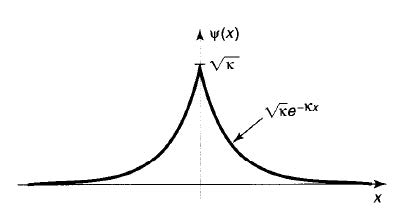
\includegraphics[width=12cm]{figure2-1.jpg}
        \caption{$\delta$函数势的束缚态波函数}
        \label{figure2.1}
    \end{figure}

    现在来讨论一下为何通常情况下波函数的导数是连续的。基本思想是对薛定谔方程从$-\varepsilon$到$\varepsilon$积分,然后取$\varepsilon \to 0$的极限
    \begin{equation}
        -\frac{\hbar^{2}}{2 m} \int_{-\varepsilon}^{\varepsilon} \frac{\dif^{2} \psi}{\dif x^{2}} \dif x+\int_{-\varepsilon}^{\varepsilon} V(x) \psi(x) \dif x=E \int_{-\varepsilon}^{\varepsilon} \psi(x) \dif x
    \end{equation}

\noindent 第一个积分是$\frac{\mathop{}\!\mathrm{d} \psi}{\mathop{}\!\mathrm{d} x}$,并在两个端点处取值;最后一个积分在$\varepsilon \to 0$极限下为零,因为它是一个高度有限宽度为零的长条的面积。这样
\begin{equation}
    \Delta \left(\frac{\mathop{}\!\mathrm{d}  \psi }{\mathop{}\!\mathrm{d} x}\right) = \left.\frac{\partial \psi}{\partial x}\right|_{+\varepsilon}-\left.\frac{\partial \psi}{\partial x}\right|_{-\varepsilon}=\frac{2 m}{\hbar^{2}} \lim _{\varepsilon \rightarrow 0} \int_{-\varepsilon}^{\varepsilon} V(x) \psi(x) \mathop{}\!\mathrm{d}  x
\end{equation}

\noindent 一般的,右边的极限也是零,这就是在通常情况下一阶导数是连续的原因。但是,当$V(x)$在边界上是无穷大时,这个结论不再成立。但可以利用这个式子得到第二个边界条件方便求解。

    回到束缚态的问题,令$\kappa = \frac{m \alpha}{\hbar^2}$,得到允许的能量值
    \begin{equation}
        E = -\frac{\hbar^2 \kappa^2}{2m} = -\frac{m \alpha^2}{2 \hbar^2}
    \end{equation}

\noindent 最后进行归一化,为了方便起见,选择正的实根,显然对于$\delta$函数势阱,无论它的“强度”$\alpha$如何,仅有一个束缚态
\begin{equation}
    \psi(x) = \frac{\sqrt{m \alpha}}{\hbar} e^{-m \alpha |x| / \hbar}; \qquad E= - \frac{m \alpha^2}{2 \hbar^2}
\end{equation}

    现在考虑散射态$E>0$的情况。这个时候对$x<0$求解,令$k = \frac{\sqrt{2 m E}}{\hbar}$(由薛定谔方程可知这是正实数),一般解为
    \begin{equation}
        \psi(x) = A e^{i k x} + B e^{ikx}
    \end{equation}

\noindent 这两项都不能丢掉。同理对于$x>0$的时候也可以得到这样形式的一般解,假设常数为$G$和$F$。将$k$也视为未知数会发现有五个变量,由于该态无法归一化,所以无法直接求解出。

    现在考虑一下这些常数的物理意义,由于$e^{\pm i k x}$分别对应于向右和向左传播的波,这样得到对应的常数正好是向右和向左传播的波的振幅。在通常的散射实验中,粒子是由一个方向入射的,在这种情况下,粒子从另外一个方向过来的波的振幅将为0,由此可以消去一些项,这样便可以求解了。

    考虑向右射入的情况(即$G=0$),可以得到
    \begin{equation}
        \begin{aligned}
            B &= \frac{i \beta}{1 - i \beta} A \\
            F &= \frac{1}{1-i \beta} A
        \end{aligned}
    \end{equation}

\noindent 则入射粒子将被反射回的相对几率是
\begin{equation}
    R = \frac{|B|^2}{|A|^2} = \frac{\beta^2}{1+\beta^2}
\end{equation}

\noindent $R$被称为\textbf{反射系数}。同样可以得到\textbf{透射系数}
\begin{equation}
    T = \frac{|F|^2}{|A|^2} = \frac{\beta^2}{1 +\beta^2}
\end{equation}

\noindent 可以看出,能量越高,透射几率越大,这当然是合理的。

    但存在一个原则上的棘手问题:这些散射波函数是不可归一化的,所以它们实际上不代表可能的粒子态。和自由粒子是一样,通过构造定态解的可归一化的线性叠加得到可归一化的解。尽管原理上直截了当,但是实际上做起来却不太容易,此时使用计算机也许是最好的方法。另外,如果不涉及能量的一个范围,构造可归一化的自由粒子波函数是不可能的,$R$和$T$应当被理解为粒子的能量在$E$附近时的近似的反射和透射系数。

    有件事容易引起困惑:我们怎么能够用定态去分析一个本质上是含时的问题:粒子入射过来,被势散射,然后又回到无限远处?我们先看一下$\varphi$,这只是一个复的、不依赖时间的正弦函数,在两个方向上都扩展(有着常数振幅)到无限远;同时,对这个波函数加上适当的边界条件,我们能够决定一个粒子(用一个局域化的波包表示)被势反射或透射的几率。隐藏在这个奇怪现象的背后的数学秘密是,通过分布在整个空间态的线性叠加以及通常的行波时间依赖关系,我们可以构造局域在一点(运动着的)相当完善的时间行为的波函数。从中可以发现,在波这个角度,时间和空间具有某种情况的对立统一特性,似乎就隐含着时空的秘密。

    最后来简短地讨论一下$\delta$函数势垒情况,如\autoref{figure2.2}所示。形式上,我们只需要改变$\alpha$前的-号为+号,当然这样一来束缚态就不存在了。另一方面,由于反射和透射系数是依赖于$\alpha^2$的,这意味着它们不会发生改变。这也就是说,粒子越过势垒就像它通过势阱一样。这意味着即便是能量小于最高势能的情况,粒子也有越过势垒的几率,这种现象被称为\textbf{隧道效应},这使得许多现代电子学技术成为可能的基础。

    \begin{figure}[htb]
        \centering
        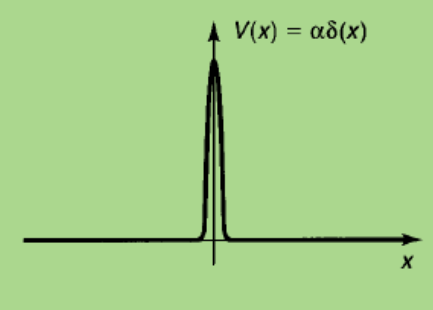
\includegraphics[width=8cm]{figure2-2.png}
        \caption{$\delta$ 函数势垒}
        \label{figure2.2}
    \end{figure}

    \subsection{有限深方势阱}
    最后来考虑有限深方势阱:
    \begin{equation}
        V(x) = \left \{ \begin{aligned}
            &-V_0, \qquad -a<x<a \\
            &0,\qquad \qquad |x|>a
        \end{aligned} \right.
    \end{equation}

    其中,$V_0>0$. 同$\delta$函数势阱一样,这个势允许有束缚态以及散射态。首先来看束缚态
    \begin{figure}[htb]
        \centering
        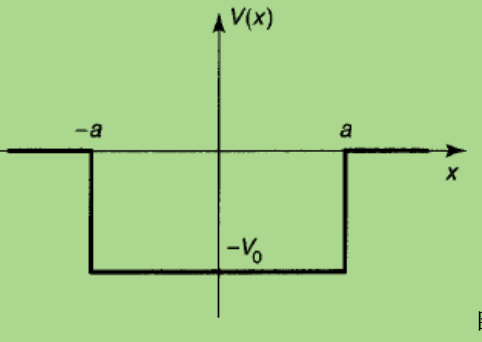
\includegraphics[width=8cm]{figure2-3.png}
        \caption{有限深方势阱}
        \label{figure2.3}
    \end{figure}

    利用薛定谔方程可以得到一般解
    \begin{equation}
        \psi(x) =A \exp(-\kappa x) + B \exp(\kappa x) 
    \end{equation}

\noindent 其中,$\kappa = \frac{\sqrt{-2mE}}{\hbar}$. 但是,当$x \to - \infty$时,解得第一项趋向于无穷大,所以物理所许可的解为
\begin{equation}
    \psi(x) = B \exp(\kappa x), \qquad x<-a
\end{equation}

    同理在$x>a$的区域里,由于存在$x \to \infty$的情况,所以物理所许可的解为
    \begin{equation}
        \psi = F \exp(-\kappa x)
    \end{equation}

    而在势阱所在的区域,即$-a < x < a$时,对于束缚态,$E> - V_0$,得到一般解
    \begin{equation}
        \psi(x) = C \sin(lx) + D \cos(lx), \qquad -a <x <a
    \end{equation}

\noindent 接下来就是利用在边界处波函数以及波函数的导数连续这样的边界条件来确定这些常数了,还有利用归一化条件。注意到势能是一个偶函数,这意味着解要不是奇函数要不是偶函数,由此可以仅需要考虑一边的边界条件,由于$\psi(-x) = \pm \psi(x)$,另一边自动满足边界条件。

    \section{形式理论}
    \subsection{希尔伯特空间}
    波函数和算符是量子理论的两块基石,其中波函数对应着体系状态,算符对应着可观察量。从数学上讲,波函数满足抽象矢量的定义形式,算符则是作为线性变换作用于矢量之上。因此,量子力学的自然语言是\textbf{线性代数}。但是这并不是一个容易熟悉的形式,需要建立从函数(波函数)到无穷维度下的矢量(右矢)的一种连接。

    对波函数可以先从N维矢量进行理解,则内积和算符运算都可以从三维矢量进行推广,注意内积运算得到的是一个复数,前面的量的分量使用的是其共轭。

    矢量的观点是一种很直观的理解方式,但需要注意,在量子力学中遇到的“矢量”是函数,它们存在于无穷维空间中,对它们进行操作要考虑到内积是否存在的问题。于是我们做一个限制,考虑到可能的物理状态,波函数都是必须归一化的
    \begin{equation}
        \int |\psi|^2 \mathop{}\!\mathrm{d} x =1 
    \end{equation}

\noindent 所有在特定区域内平方可积的函数的集合构成一个(非常小)的矢量空间,物理学家称它为\textbf{希尔伯特空间},从这个角度上说,\red{波函数是处于希尔伯特空间中的}。

    定义两个函数$f(x),g(x)$的内积如下
    \begin{equation}
        \langle f | g \rangle = \int_{a}^{b} f(x)^* g(x) \mathop{}\!\mathrm{d} x
    \end{equation}

\noindent 如果f和g都是平方可积的,那么它们的内积将肯定存在,这可由史瓦西不等式得出
\begin{equation}
    \left|\int_{a}^{b} f(x)^{*} g(x) \mathop{}\!\mathrm{d}  x\right| \leq \sqrt{\int_{a}^{b}|f(x)|^{2} d x \int_{a}^{b}|g(x)|^{2} \mathop{}\!\mathrm{d}  x}
    \end{equation}

\noindent 容易看出,与自己的内积是一个非负实数,当且只当本身为零时内积为零。

    如果一个函数与自身的内积为1,则称之为\textbf{归一化的};如果两个函数的内积为0,那么这两个函数是\textbf{正交的}。

    最后,如果存在一组函数,其他任意函数(希尔伯特空间中)都可以表示为这组函数的线性叠加,那么这组函数是\textbf{完备}的,可以理解为是希尔伯特空间的基矢
    \begin{equation}
        f(x) = \sum_{n=1}^{\infty} c_n f_n(x)
    \end{equation}

\noindent 如果这一组函数是正交归一的,即每一个函数都是正交的,任意两个函数之间是归一的,则上式的常数可以有傅里叶技巧得到
\begin{equation}
    c_n = \langle f_n | f \rangle
\end{equation}

    \subsection{可观测量}
    \subsubsection{厄米算符}
    一个可观察量$Q(x,p)$的期望值可以用内积符号简洁表示出来:
    \begin{equation}
        \langle Q\rangle=\int \psi^{\prime} \hat{Q} \psi \mathop{}\!\mathrm{d}  x=\langle\psi | \hat{Q} \psi\rangle
        \end{equation}

\noindent 每一次测量的结果应该是实数,多次测量的平均值理应也是实数,这意味着
\begin{equation}
    \langle Q \rangle = \langle Q \rangle^*
\end{equation}

\noindent 但内积的复共轭运算颠倒了顺序
\begin{equation}
    \langle\psi | \hat{Q} \psi\rangle=\langle\hat{Q} \psi | \psi\rangle
    \end{equation}

\noindent 任意波函数都满足此式。因此表示可观察量的算符具有非常特殊的性质,定义如果存在对任何$f(x)$,都有
\begin{equation}
    \langle f | \hat{Q} f\rangle=\langle\hat{Q} f | f\rangle
    \end{equation}

\noindent 成立的算符,即为\textbf{厄米算符}。与之等价的定义是满足
\begin{equation}
    \hat{Q} = \hat{Q}^*
\end{equation}

\noindent 的算符被称为厄米算符。这个等式一般写作$\hat{Q}^{\dagger} = \hat{Q}$.

    容易得知,在量子力学中,\red{可观察量由厄米算符表示}。

    \subsubsection{定值态}
    可以制备一个态$\Psi_n(x,t)$,对应于一个可观察量$\hat{Q}$,得到定值q,这意味着对于这个算符,在定值态下得到的标准差应该是0
    \begin{equation}
        \sigma^{2}=\left\langle(\hat{Q}-\langle Q\rangle)^{2}\right\rangle=\left\langle\Psi |(\hat{Q}-q)^{2} \Psi\right\rangle=\langle(\hat{Q}-q) \Psi |(\hat{Q}-q) \Psi\rangle= 0
        \end{equation}

\noindent 所以
\begin{equation}
    \hat{Q} \Psi = q \Psi
\end{equation}

\noindent 这称为算符$\hat{Q}$的本征值方程;$\Psi$是$\hat{Q}$的一个本征函数,q是对应的本征值,因此,\red{定值态是$\hat{Q}$的本征函数}。

    注意到本征值是一个数——既不是算符也不是函数,所以任意本征函数乘以一个常数,依然是一个具有相同本征值的本征函数。这里要排除零,它不属于本征函数,不然对于所有的算符和本征值它都是成立的,这事没有意义的。然而,零作为本征值却是恰当的。一个算符所有的本征值的集合称为这个算符的\textbf{谱},在后面你们会看到所谓的\textbf{分离谱}和\textbf{连续谱},其中谱的意思都是这个。有的时候两个或者更多\textbf{线性独立}的本征函数具有相同的本征值,这种情况下称作谱的\textbf{简并}。在量子力学中,简并是一个十分重要的概念。

    \subsection{厄米算符的本征函数}
    对于某一厄米算符的本征函数,可分为两种情况:如果谱是分立的,则本征函数处于希尔伯特空间中并且构成物理上可实现的态;如果谱是连续的,即本征值充满一个范围,那么本征函数是不可归一化的,并且它们不可能代表可能的波函数(尽管它们的线性叠加——这必定包括本征值的一个分布——可能是可归一化的)。某些算符仅有分立谱,某些算符仅有连续谱,还有一些既具有分立谱也有连续谱。

    \subsubsection{分立谱}
    数学上厄米算符可归一化的本征函数具有三个重要性质,证明都十分简单(第三个实际上没法证明,在N维空间下的可以通过线性代数相关知识证明,不幸的是,它无法推广到无穷维的空间中,所以在量子力学中将其视作一个公立,或者更确切的理解是,看作是\red{加在表示可观察量的厄米算符上的一个限制条件})
    \begin{itemize}
        \item 本征值是实数
        \item 属于不同本征值的本征函数是正交的
        \item 这些函数张成空间(即是完备的)
    \end{itemize}

\noindent 这个性质非常重要,以后很多问题得到的解都可以由此知道定态解是相互正交的。

    不过可惜,定理2没有告诉我们任何关于简并态的情况。然而,幸运的是,如果两个本征函数具有相同的本征值,任何它们线性的组合依然是具有同样本征值的本征函数,而且,在每一个简并的子空间内,我们都可以利用Gram-Schmidt正交化步骤构建相互正交的本征函数,在原则上总是可以做到的。所以,即使存在简并,本征函数依然可以选择彼此正交,这就允许我们依据基函数的正交归一性使用傅里叶技巧。

    \subsubsection{连续谱}
    如果一个厄米算符的谱是连续的,由于内积可能不存在,其本征函数是不可归一化的,因而前面三个性质的前两个的证明是没法成立的。然而,在某种意义上这三个基本的性质依然成立。

    以动量算符为例,假设$f_p(x)$是本征函数,$p$是本征值
    \begin{equation}
        \frac{\hbar}{i} \frac{\mathop{}\!\mathrm{d} }{\mathop{}\!\mathrm{d} x} f_p(x) = pf_p(x)
    \end{equation}

\noindent 一般解是
\begin{equation}
    f_p(x) = A e^{i p x/ \hbar}
\end{equation}

\noindent 对于任何(复数的)p值,它都不是平方可积的——动量算符在希尔伯特空间没有本征函数。然而,如果我们限定于实数本征值,可以得到一个人为的“正交归一性”。可以发现,实际上我们要考虑的问题即是本征值为实数的情况——与此对应的是物理上存在的态,所以其实不用慌,问题不大。注意到
\begin{equation}
    \int_{\infty}^{\infty} f_{p^{\prime}}^{*}(x) f_{p}(x) \mathop{}\!\mathrm{d}  x=|A|^{2} \int_{-\infty}^{\infty} e^{i\left(p-p^{\prime}\right) x / \hbar} \mathop{}\!\mathrm{d}  x=|A|^{2} 2 \pi \hbar \delta\left(p-p^{\prime}\right)
    \end{equation}

    如果我们取$A = \frac{1}{\sqrt{2 \pi \hbar}}$,有 
    \begin{equation}
        f_p(x) = \frac{1}{\sqrt{2 \pi \hbar}} e^{i p x / \hbar}
    \end{equation}

\noindent 那么
\begin{equation}
    \langle f_{p^{\prime}}| f_p \rangle = \delta (p - p^{\prime})
\end{equation}

\noindent 明显让人联想到真正的正交归一性。这个符号便是著名的\textbf{狄拉克符号},因而我们不妨称之为\textbf{狄拉克正交归一性}。

    最重要的是,其本征函数是完备的,不过使用一个积分代替了求和:任何(平方可积的)函数——即存在于希尔伯特空间中的——都可以写作下列形式
    \begin{equation}
        f(x)=\int_{-\infty}^{\infty} c(p) f_{p}(x) \mathop{}\!\mathrm{d}  p=\frac{1}{\sqrt{2 \pi \hbar}} \int_{-\infty}^{\infty} c(p) e^{i p x / \hbar} \mathop{}\!\mathrm{d}  p
        \end{equation}

    仍然可以利用傅里叶技巧得到展开系数,只不过现在是一个有关p的函数
    \begin{equation}
        \left\langle f_{p^{\prime}} | f\right\rangle=\int_{-\infty}^{\infty} c(p)\left\langle f_{p^{\prime}} | f_{p}\right\rangle \mathop{}\!\mathrm{d}  p=\int_{-\infty}^{\infty} c(p) \delta\left(p-p^{\prime}\right) \mathop{}\!\mathrm{d}  p=c\left(p^{\prime}\right)
        \end{equation}

    注意到在动量算符作用下本征值为实数的那些本征态依旧不会是实际可能的物理态,实际的物理态都是对这些本征态的在一定分布下的求和,再考虑到这个动量算符对应的本征函数是正弦函数,波长为
    \begin{equation}
        \lambda = \frac{2 \pi \hbar}{p}
    \end{equation}

\noindent 这正是德布罗意公式,所以这个动量算符得到的是自由粒子的动量,这意味着对于自由粒子来说,不存在一个确定的动量。这体现了量子力学的一个重要的观点,对于自由粒子来说,实际上存在的是一个波包,其动量分布在一个范围之中。

    对于位置算符来说可以得到类似的结果,这说明对于自由粒子来说也不存在一个确定的位置,位置分布在一个范围之中,从这已经能初步窥探到不确定性原理了。

    总结一下,如果厄米算符的谱是连续的,本征函数是不可归一化的,它们不在希尔伯特空间并且不能代表可能的物理态;然而,具有实数本征值的本征函数具有狄拉克正交归一性,并且是完备的(区别只在于分立时是求和而现在是积分)。幸运的是,这正是我们所需要的。

    \subsection{广义统计诠释}
    广义统计诠释可以告诉我们如何任何测量测量的可能结果并让我们计算出出现这些结果的几率。广义统计诠释内容如下:

    如果测量一个处于$\Psi(x,t)$态的粒子的可观测量$Q(x,p)$,那么,其结果一定是厄米算符$\hat{Q}(x,-i \hbar \frac{\mathop{}\!\mathrm{d} }{\mathop{}\!\mathrm{d} x})$的一个本征值。如果$\hat{Q}$的谱是分立的,得到与正交归一本征函数$f_n(x)$相应的本征值$q_n$的几率是$|c_n|^2$,其中$c_n = \langle f_n | \Psi \rangle$. 如果$\hat{Q}$的谱是连续的,具有实数本征值$q(z)$的几率是$|c(z)|^2 \mathop{}\!\mathrm{d} z$,其中$c(z) = \langle \langle f_z | \Psi \rangle$. 测量后,波函数“坍缩”于相应的本征态。

    统计诠释帮助我们更好地理解:一个可观察量的本征函数是完备的,所以波函数可以写作它们的线性叠加。由于本征函数是正交归一的,展开系数可由傅里叶技巧得出。注意不要简单地将系数理解为\textbf{$\Psi$里中包含有多少$f_n$},因为几率是由波函数的模平方决定的,其精确度实际上是$|c_n|^2$. 这才是广义统计诠释的精髓所在。

    容易证明,总的几率必须是1,对于一可观察量$\hat{Q}$的期望值应该是任何可能性的本征值与本征值出现几率的乘积的求和。

    从这个角度再来考虑完备性,可以得知:任何实际态都可写作这些完备本征态的线性叠加,系数的平方即所对应本征值的几率。总的几率为1.

    特别地,测量一个处于$\Psi$态的粒子的位置其结果一定是坐标算符的本征值。由于每个实数y均为位置本征函数$g_y(x) = \delta(x-y)$的本征值,所以
    \begin{equation}
        c(y) = \langle g_y | \Psi \rangle = \Psi(y,t)
    \end{equation}

\noindent 自然在某一范围$\mathop{}\!\mathrm{d} y$出现的概率即为$|\Psi(y,t)|^2 \mathop{}\!\mathrm{d} y$.

    类似地,动量算符本征函数
    \begin{equation}
        f_p(x) = \frac{1}{\sqrt{2 \pi \hbar}}\int_{-\infty}^{\infty}e^{-ipx/\hbar}
    \end{equation}

\noindent 所以,$c(p) = \langle f_p | \Psi \rangle = \frac{1}{\sqrt{2 \pi \hbar}}\int_{-\infty}^{\infty}e^{-ipx/\hbar} \Psi(x,t) \mathop{}\!\mathrm{d} x$. 这是很重要的一个量,被称为\textbf{动量空间波函数},它和位置空间波函数(简称“波函数”)之间可通过傅里叶变换得到
\begin{equation}
\begin{array}{l}{\Phi(p, t)=\frac{1}{\sqrt{2 \pi \hbar}} \int_{-\infty}^{\infty} e^{-i p x / \hbar} \Psi(x, t) \mathop{}\!\mathrm{d}  x} \\ {\Psi(x, t)=\frac{1}{\sqrt{2 \pi \hbar}} \int_{-\infty}^{\infty} e^{-i p x / \hbar} \Phi(p, t) \mathop{}\!\mathrm{d}  p}\end{array}
\end{equation}

\noindent 原则上,可以像再坐标空间一样再动量空间进行所有的计算,只不过不是都很简便。
\begin{equation}
\langle Q(x, p)\rangle=\left\{\begin{array}{l}{\int \Psi^{*} \hat{Q}\left(x, \frac{\hbar}{i} \frac{\partial}{\partial x}\right) \Psi \mathop{}\!\mathrm{d}  x} \\ {\int \Phi^{*} \hat{Q}\left(-\frac{\hbar}{i} \frac{\partial}{\partial p}, p\right) \Phi \mathop{}\!\mathrm{d}  p}\end{array}\right.
\end{equation}

    事实上,这也正是动量表象和坐标表象——其实表象可以理解为一个空间,它是对所要研究的对象在某一特定角度的描述,得到的可观察量理应是相同的。

    \subsection{不确定性原理}
    对于任意一可观察量,我们有
    \begin{equation}
        \sigma^2_A = \langle (\hat{A} - \langle A \rangle) \Psi | (\hat{A}- \langle A \rangle )\Psi \rangle = \langle f | f \rangle
    \end{equation}

\noindent 式中$f \equiv (\hat{A} - \langle A \rangle ) \Psi$. 同样地,对于任何另外一个可观察量,有
\begin{equation}
    \sigma_B^2 = \langle g | g \rangle 
\end{equation}

\noindent 其中,$g \equiv (\hat{B} - \langle B \rangle ) \Psi$,因此根据史瓦西不等式,有
\begin{equation}
    \sigma_{A}^{2} \sigma_{B}^{2}=\langle f | f\rangle\langle g | g\rangle \geq|\langle f | g\rangle|^{2} \label{equ3.1}
    \end{equation}

    而对于任意一个复数z,有
    \begin{equation}
        |z|^{2}=[\operatorname{Re}(z)]^{2}+[\operatorname{Im}(z)]^{2} \geq[\operatorname{Im}(z)]^{2}=\left[\frac{1}{2 i}\left(z-z^{*}\right)\right]^{2}\label{equ3.2}
        \end{equation}

\noindent 因此,令$z = \langle f | g \rangle $
\begin{equation}
    \sigma_A^2 \sigma_B^2 \ge \left(\frac{1}{2i}\left[\langle f| g \rangle  - \langle g|f \rangle \right]\right)^2
\end{equation}

\noindent 容易证明
\begin{equation}
    \langle f | g \rangle  = \langle \hat{A} \hat{B}\rangle - \langle \hat{A} \rangle \langle \hat{B} \rangle  
\end{equation}

\noindent 类似有
\begin{equation}
    \langle g|f \rangle  = \langle \hat{B}\hat{A} \rangle -\langle \hat{A} \rangle \langle \hat{B} \rangle
\end{equation}

\noindent 所以得到\textbf{普遍的不确定性原理}
\begin{equation}
    \sigma_{A}^{2} \sigma_{B}^{2} \geq\left(\frac{1}{2 i}\langle[\hat{A}, \hat{B}]\rangle\right)^{2} \label{equ3.5}
    \end{equation}

    海森堡不确定性原理只是这个更普遍理论的一个应用而已。事实上,对每一对其算符不対易的可观察量都存在一个“不确定性原理”——我们称它们为\textbf{不相容可观测量}。不相容可观测量没有共同的本征函数——至少(这是可以证明的),它们不能有完备的本征函数系。

    不确定性原理是统计诠释的结果,测量坍缩特性为其提供了操作保障,而只有两个可观测量是对易时,测量导致体系的坍缩才不会影响到两者的测量。

    \subsubsection{最小不确定波包}
    什么是最一般的最小不确定波包呢?回望不确定性原理的证明,有两个地方用了不等式:\autoref{equ3.1}\\
    和\autoref{equ3.2}. 现在我们将它们变为等式,看看能从中告诉我们$\Psi$的哪些信息。
    对于\autoref{equ3.1},变成等式意味着两者存在倍数关系,即$g(x) = cf(x)$,其中的$c$为特定的复数。对于\autoref{equ3.2},要变成等式意味着z为纯虚数,这要求$\operatorname{Re} \langle f|g \rangle = \operatorname{Re} \left( c \langle f|f \rangle \right)= 0$. 由于$\langle f|f \rangle $必是实数,这就意味着常数c必须是纯虚数——我们将它表示为$ia$. 因此,对最小不确定成立的充分必要条件为
    \begin{equation}
        g(x) = ia f(x)
    \end{equation}

\noindent 其中,$a$为实数。

    对于坐标—动量不确定性原理来说这个判据为
    \begin{equation}
        \left(\frac{\hbar}{i}\frac{\mathop{}\!\mathrm{d} }{\mathop{}\!\mathrm{d} x} - \langle p \rangle \right) \Psi = ia (x-\langle x \rangle ) \Psi
    \end{equation}

\noindent 这是一个作为$x$的函数的微分方程,其一般解为
\begin{equation}
    \Psi(x)=A e^{-a(x-\langle x\rangle)^{2} / 2 \hbar} e^{i\langle p\rangle x / \hbar}
    \end{equation}

\noindent 显然,最小不确定波包是一个高斯波包。由于方程中存在可能和时间有关的数,这种情况下波函数会演变而偏离最小形式。但能够确定的是,在某个时候波函数是x的高斯函数的时候,不确定之积是最小的。

    \subsubsection{能量-时间不确定原理}
    在狭义相对论中,$\Delta t \Delta E \ge \frac{\hbar}{2}$可以视为坐标动量版本的一个推论,这是由于$x$和$ct$、$p$和$\frac{E}{c}$在坐标-时间4-矢量与能量-动量4-矢量里一同变换。

    然而,薛定谔方程是非相对论的,我们一直考虑的也是非相对论性的量子力学,所以在此框架下这两个不确定原理没有太紧密的联系,虽然表面上显得很相似。注意时间是一个独立变量,它本身不是动力学变量(在任何情况下,在非相对论中都不是),动力学量是它的函数。特别地,能量-时间不确定原理中的$\Delta t$不是对时间测量所收集数据的标准差;粗略地讲,正是时间让体系发生实质性的变化。

    当测量一个体系变化有多快时,我们来求某个可观察量的期望值对时间的导数,对于可观察量$\hat{Q}(x,p,t)$
    \begin{equation}
        \frac{\mathop{}\!\mathrm{d} }{\mathop{}\!\mathrm{d}  t}\langle Q\rangle=\frac{\mathop{}\!\mathrm{d} }{\mathop{}\!\mathrm{d}  t}\langle\Psi | \hat{Q} \Psi\rangle=\left\langle\frac{\partial \Psi}{\partial t} | \hat{Q} \Psi\right\rangle+\left\langle\Psi | \frac{\partial \hat{Q}}{\partial t} \Psi\right\rangle+\left\langle\Psi | \hat{Q} \frac{\partial \Psi}{\partial t}\right\rangle
        \end{equation}

\noindent 由薛定谔方程
\begin{equation}
    i \hbar \frac{\partial \Psi}{\partial t} \hat{H} \Psi
\end{equation}

\noindent 所以
\begin{equation}
    \frac{\mathop{}\!\mathrm{d} }{\mathop{}\!\mathrm{d}  t}\langle Q\rangle=-\frac{1}{i \hbar}\langle\hat{H} \Psi | \hat{Q} \Psi\rangle+\frac{1}{i \hbar}\langle\Psi | \hat{Q} \hat{H} \Psi\rangle+\left\langle\frac{\partial \hat{Q}}{\partial t}\right\rangle
    \end{equation}

\noindent 由于$\hat{H}$是厄米算符,$\langle \hat{H} \Psi | \hat{Q} \Psi \rangle  = \langle \Psi | \hat{H} \hat{Q} \Psi \rangle $,所以有
\begin{equation}
    \frac{d}{d t}\langle Q\rangle=\frac{i}{\hbar}\langle[\hat{H}, \hat{Q}]\rangle+\left\langle\frac{\partial \hat{Q}}{\partial t}\right\rangle
    \end{equation}

\noindent 在算符不显含时间的通常情况下,它告诉我们算符期望值的变化率决定于此算符与哈密顿量的对易式。特别地,如果$\hat{Q}$与$\hat{H}$对易,则$\langle \hat{Q} \rangle $是常量,在这个意义上是一个守恒量。

    回到不确定性原理之中,假设$\hat{Q}$不显含时间,可以得到
    \begin{equation}
        \sigma_{H}^{2} \sigma_{Q}^{2} \geq\left(\frac{1}{2 i}\langle[\hat{H}, \hat{Q}]\rangle\right)^{2}=\left(\frac{1}{2 i} \frac{\hbar}{i} \frac{\mathop{}\!\mathrm{d} \langle Q\rangle}{\mathop{}\!\mathrm{d}  t}\right)^{2}=\left(\frac{\hbar}{2}\right)^{2}\left(\frac{\mathop{}\!\mathrm{d} \langle Q\rangle}{\mathop{}\!\mathrm{d}  t}\right)^{2}
        \end{equation}

\noindent 即
\begin{equation}
    \sigma_H \sigma_Q \ge \frac{\hbar}{2} \left| \frac{\mathop{}\!\mathrm{d} \langle \hat{Q} \rangle }{\mathop{}\!\mathrm{d} t}\right|
\end{equation}

    我们定义$\Delta E \equiv \sigma_H$和
    \begin{equation}
        \Delta t \equiv \frac{\sigma_Q}{|\mathop{}\!\mathrm{d} \langle \hat{Q} \rangle / \mathop{}\!\mathrm{d} t|}
    \end{equation}

\noindent 则有
\begin{equation}
    \Delta E \Delta t \ge \frac{\hbar}{2}
\end{equation}

\noindent 这就是能量-时间不确定原理,但请注意下面两点:
\begin{itemize}
    \item 能量-时间不确定原理更多是个定义,对什么叫$\Delta t$的定义
    \item $\Delta t$完全依赖于可观察量的情况,但当$\Delta E$很小时,所有的可观察量变化得都比较平缓;反过来说,可观察量变化很快时,能量的不确定性很大
\end{itemize}

    \subsection{狄拉克符号}
    量子力学中的态用希尔伯特空间的右矢表示(设为$\langle a \rangle$),但是我们可以用不同的基来表示它——即右矢唯一,表象,或者说,描述方法不唯一。联想普通的矢量空间可以理解,在空间里的矢量是客观存在的,但可以选择不同的基矢,或者说坐标系去对它进行描述。基矢的不同使得分量的表示不同,但指代的都是同一个矢量。

    波函数其实是用坐标的本征函数作为基矢时对右矢的描述,具体为用坐标的本征函数对右矢进行展开时的系数
    \begin{equation}
        \Psi(x,t) = \langle x | a \rangle 
    \end{equation}

    类似地,动量波函数是用动量的本征函数作为基矢时对右矢的描述
    \begin{equation}
        \Phi(p,t) = \langle x|a \rangle 
    \end{equation}

    也可以用能量的本征函数作为基矢对其进行展开
    \begin{equation}
        c_n(t) = \langle n|a \rangle 
    \end{equation}

    这些描述的是同一个态,相互可以进行转换
    \begin{equation}
    \begin{aligned} \Psi(x, t) &=\int \Psi(y, t) \delta(x-y) \mathop{}\!\mathrm{d}  y \\ &=\int \Phi(p, t) \frac{1}{\sqrt{2 \pi \hbar}} e^{i p x / \hbar} \mathop{}\!\mathrm{d}  p \\ &=\sum c_{n} e^{i E_n t / \hbar} \psi_{n}(x) \end{aligned}
    \end{equation}

    表示可观察量的算符是一种线性变换——把一个矢量变换到另一个,所以算符的作用是对态进行改变。但对于该算符的本征函数,由于结果是在这个函数前面乘上一个常数——在量子力学所采用的数学中,矢量(即右矢)前面的系数不是区别态的依据,即右矢的方向不包含信息——所以并没有改变态。这对应物理上的一个现象:当进行观测之后,态坍缩本征态,这时再进行同样的测量得到的结果是恒定的,即态不会发生改变,稳定在第一次观测后坍缩而成的本征态上。

    对某组基,算符是用矩阵来表示的,对应的矩阵元为
    \begin{equation}
        \langle e_m|\hat{Q}e_n \rangle  = Q_{mn}
    \end{equation}

\noindent 因而右矢和算符的相关计算均可完全仿照线性代数。

    右矢是一个矢量,那现在问题来了,左矢对应的是什么?我们发现,左矢和右矢合作后可以生成一个数(一般是复数),而且满足线性关系,这意味着左矢应该是右矢的一个线性泛函:
    \begin{equation}
        \langle f | = \int f^* [\cdots] \mathop{}\!\mathrm{d} x
    \end{equation}

\noindent 其中$\cdots$表示右矢。所有的左矢集合构成了另外一个矢量空间——对偶空间。

    有一种特殊的算符
    \begin{equation}
        \hat{P} = | \alpha \rangle \langle \alpha |
    \end{equation}

\noindent 将会从任意其他矢量中选出沿着$| \alpha \rangle$方向的部分
\begin{equation}
    \hat{P}| \beta \rangle = \langle \alpha | \beta \rangle | \alpha \rangle
\end{equation}

\noindent 被称为向$| \alpha \rangle$张成的一维子空间的投影算符。

特别地,如果$\{| e_n \rangle\}$是一分立的正交归一基
\begin{equation}
    \langle e_m | e_n \rangle = \delta_{mn}
\end{equation}

\noindent 那么可以得到
\begin{equation}
    \sum_{n} | e_m \rangle \langle e_n | =1 \label{equ3.3}
\end{equation}

    类似地,$\{| e_z \rangle\}$是一狄拉克正交归一的连续基
    \begin{equation}
        \langle e_z | e_{z^{\prime}} \rangle = \delta(z-z^{\prime})
    \end{equation}

\noindent 那么可以得到
\begin{equation}
    \int | e_z \rangle \langle e_{z^{\prime}} \mathop{}\!\mathrm{d} z =1 \label{equ3.4}
\end{equation}

    注意,\autoref{equ3.3}和\autoref{equ3.4}是表达完备性最简洁的形式——任何矢量由它们进行展开都可以得到矢量本身。

    \section{三维空间中的量子力学}
    \subsection{球坐标下的薛定谔方程}
    在球坐标下薛定谔方程可以写作
    \begin{equation}
        i \hbar \frac{\partial \Psi}{\partial t} = \frac{\hbar^2}{2m} \nabla^2 \Psi + V \Psi 
    \end{equation}
    
\noindent 其中
\begin{equation}
    \nabla^2 \equiv \frac{1}{r^2} \frac{\partial}{\partial r} \left(r^2 \frac{\partial}{\partial r}\right) + \frac{1}{r^2} \frac{1}{\sin \theta} \frac{\partial}{\partial \theta}\left(\sin \theta \frac{\partial}{\partial \theta}\right) + \frac{1}{r^2} \frac{1}{\sin^2 \theta}  \left(\frac{\partial^2}{\partial \phi^2}\right)
\end{equation}

\noindent 被称为拉普拉斯算符。

    归一化现在是对于体元进行积分
    \begin{equation}
        \int \int \mathop{}\!\mathrm{d} r \mathop{}\!\mathrm{d} \Omega |\Psi| =1
    \end{equation}

\noindent 其中积分是对整个空间进行。如果势不显含时间,将有一组完备的定态
\begin{equation}
    \Psi_n(\vec{r},t) = \psi_n(\vec{r}) e^{-iE_n t/\hbar}
\end{equation}

\noindent 其中空间波函数$\psi$满足定态薛定谔方程
\begin{equation}
    - \frac{\hbar^2}{2m} \nabla^2 \psi + V \psi = E \psi \label{equ4.11}
\end{equation}

    (含时)薛定谔方程的一般解为
    \begin{equation}
        \Psi(\vec{r},t) = \sum_n c_n \psi_n (\vec{r}) e^{-i E_n t/\hbar}\label{equ4.1}
    \end{equation}

\noindent 其中常数$c_n$由初始波函数用通常的方法确定。如果势允许连续态,那么\autoref{equ4.1}的求和变为积分。

    \subsubsection{分离变量法}
    只考虑不含时薛定谔方程,因为现在考虑的都是时间依赖项和位置依赖项解耦的波函数,只要求出了空间波函数最后加上$e^{- i  E_n t/\hbar}$就可以得到最终的波函数了。进一步使用分离变量法,令
    \begin{equation}
        \psi(r,\theta,\phi) = R(r) Y(\theta,\phi)
    \end{equation}

\noindent 将其代入\autoref{equ4.11}可以得到 
\begin{equation}
    -\frac{\hbar^{2}}{2 m}\left[\frac{Y}{r^{2}} \frac{\mathop{}\!\mathrm{d} }{\mathop{}\!\mathrm{d} r}\left(r^{2} \frac{\mathop{}\!\mathrm{d} R}{\mathop{}\!\mathrm{d} r}\right)+\frac{R}{r^{2} \sin \theta} \frac{\partial}{\partial \theta}\left(\sin \theta \frac{\partial Y}{\partial \theta}\right)+\frac{R}{r^{2} \sin \theta^{2}} \frac{\partial^{2} Y}{\partial \phi^{2}}\right] + V Y R = E Y R
    \end{equation}

\noindent 经过简单处理可以使得$R$ 和$Y$分离,得到
\begin{equation}
\begin{array}{l}{\left\{\frac{1}{R} \frac{\mathop{}\!\mathrm{d}}{\mathop{}\!\mathrm{d} r}\left(r^{2} \frac{\mathop{}\!\mathrm{d} R}{\mathop{}\!\mathrm{d} r}\right)-\frac{2 m r^{2}}{\hbar^{2}}[V(r)-E]\right\}} \\ {+\frac{1}{Y}\left\{\frac{1}{\sin \theta} \frac{\partial}{\partial \theta}\left(\sin \theta \frac{\partial Y}{\partial \theta}\right)+\frac{1}{\sin \theta^{2}} \frac{\partial^{2} Y}{\partial \phi^{2}}\right\}=0}\end{array}
\end{equation}

\noindent 由于解耦,可以知道两边都只能等于一个常数,由于以后会明白的理由,我们将其写作$l(l+1)$.

    \subsubsection{角动量方程}
    继续分离变量,令$Y(\theta,\phi) = \Theta(\theta)\Phi(\phi)$,只考虑和$Y$有关的那一部分,得到
    \begin{equation}
        \left\{\frac{1}{\Theta}\left[\sin \theta \frac{\mathop{}\!\mathrm{d} }{\mathop{}\!\mathrm{d}  \theta}\left(\sin \theta \frac{\mathop{}\!\mathrm{d}  \Theta}{\mathop{}\!\mathrm{d}  \theta}\right)\right]+l(l+1) \sin \theta^{2}\right\}+\frac{1}{\Phi} \frac{\mathrm{d}^{2} \Phi}{\mathrm{d} \phi^{2}}=0
        \end{equation}

\noindent 依旧是都等于一个常数,这次令其为$m^2$. 有关$\Theta$的方程非常简单,得到
\begin{equation}
    \frac{\mathop{}\!\mathrm{d}^2 \Phi}{\mathop{}\!\mathrm{d} \phi^2} = -m^2 \Rightarrow \Phi(\phi) = e^{i m \phi} \label{equ4.9}
\end{equation}

\noindent 其中,$m$可正可负,这就把两组解都包括进去了。前面还应该有个常数因子,但可以被吸收到$\Theta$中去。由于当$\theta$变化$2 \pi$时,回到了空间同一点,这很自然要求
\begin{equation}
    \Phi(\phi + 2 \pi) = \Phi(\phi)
\end{equation}

\noindent 这就要求$m$必须为整数。

    对于有关$\theta$的方程,不幸的是,解起来很困难;幸运的是,这意味着我们只需要学会查表。首先来看一下这个方程
    \begin{equation}
        \sin \theta \frac{\mathop{}\!\mathrm{d} }{\mathop{}\!\mathrm{d} \theta} \left(\frac{\mathop{}\!\mathrm{d} \Theta}{\mathop{}\!\mathrm{d} \theta}\right) + \left[l(l+1) \sin \theta^2 - m^2 \right] \Theta = 0 \label{equ4.4}
    \end{equation}

\noindent 很明显,这样的方程的解适合变成特殊函数然后让我们查表。事实上确实是如此的,这个解为
\begin{equation}
    \Theta(\theta) = A P_l^m (\cos \theta)
\end{equation}

\noindent 其中$P_l^m$被称为\textbf{缔结勒让德函数},其定义为
\begin{equation}
    P_{l}^{m}(x) \equiv\left(1-x^{2}\right)^{|m| / 2}\left(\frac{\mathop{}\!\mathrm{d} }{\mathop{}\!\mathrm{d}  x}\right)^{|m|} P_{l}(x) \label{equ4.3}
    \end{equation}

\noindent 其中$P_l(x)$是\textbf{勒让德多项式},其定义为
\begin{equation}
    P_l^m(x) \equiv \frac{1}{2^l l!} \left(\frac{\mathop{}\!\mathrm{d} }{\mathop{}\!\mathrm{d} x} \right)^l (x^2-1)^l
\end{equation}

    注意缔结勒让德函数中的自变量为$\cos \theta$. 为了使勒让德多项式的定义有意义,$l$必须是一个非负整数;另外,如果$|m| > l$,那么由方程\autoref{equ4.3}知$P_l^m=0$. 因此,对于任何给定的$l,m$,都有$(2m +1)$个不同的取值。但请注意,\autoref{equ4.4}是一个二阶方程,对于任何一组$(l,m)$,它应该有两个线性独立的解。那另外一个解呢?事实上,在数学上它们是成立的,但在物理上却是不可接受的,因为它们在$\theta = 0 || 2 \pi $时为无穷大。

    归一化条件为
    \begin{equation}
        \int |\psi|^2 r^2 \sin \theta \mathop{}\!\mathrm{d} r \mathop{}\!\mathrm{d} \theta \mathop{}\!\mathrm{d} \phi = \int |R|^2 r^2 \mathop{}\!\mathrm{d} r \int |Y|^2 \sin \theta \mathop{}\!\mathrm{d} \theta \mathop{}\!\mathrm{d} \phi = 1
    \end{equation}

\noindent 对$R$和$Y$分别归一化是方便的
\begin{equation}
    \begin{aligned}
        \int_0^{\infty} |R|^2 r^2 \mathop{}\!\mathrm{d} r&=1 \\
        \int_{0}^{2 \pi} \int_{0}^{\pi} \sin \theta \mathop{}\!\mathrm{d} \theta \mathop{}\!\mathrm{d} \phi = 1   
    \end{aligned}
\end{equation}

    \begin{figure}[htb]
        \centering
        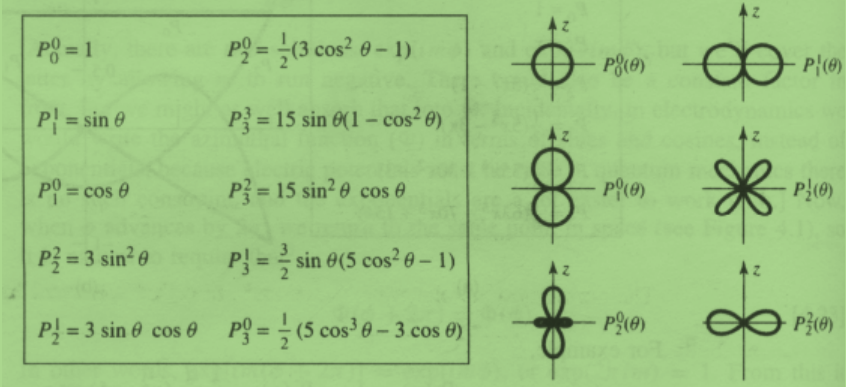
\includegraphics[width=10cm]{figure4-1.png}
        \caption{一些缔结勒让德函数的函数形式和图像形式}
        \label{figure4.1}
    \end{figure}

    归一化的角向波函数被称为\textbf{球谐函数}:
    \begin{equation}
        Y_l^m(\theta,\phi) \varepsilon \sqrt{\frac{(2l-1)(l-|m|)!}{4 \pi (l+|m|)!}} e^{im\phi} P_l^m(\cos theta)
    \end{equation}

    \begin{figure}[htb]
        \centering
        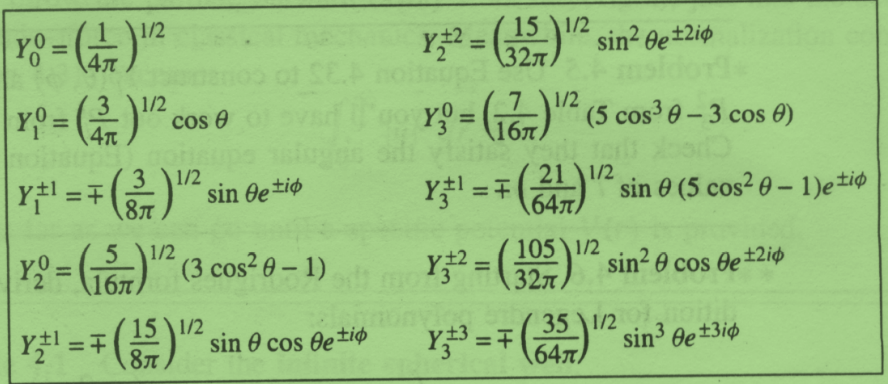
\includegraphics[width=8cm]{figure4-2.png}
        \caption{前几个球谐函数}
        \label{figure4.2}
    \end{figure}
    
\noindent 其中当$m \ge 1$时$\varepsilon = (-1)^m$,当$m \le 0$时$\varepsilon =1$. 可以证明它们是自动正交的,在后面会给出证明,所以
\begin{equation}
    \int_{0}^{2 \pi} \int_{0}^{\pi}\left[Y_{t}^{m}(\theta, \phi)\right]^{*}\left[Y_{r^{\prime}}^{m^{\prime}}(\theta, \phi)\right] \sin \theta \mathop{}\!\mathrm{d}  \theta \mathop{}\!\mathrm{d}  \phi=\delta_{ll^{\prime}} \delta_{m m^{\prime}}
    \end{equation}

\noindent 由于历史原因$l$被称为\textbf{角量子数},而$m$被称为\textbf{磁量子数}。

    \subsubsection{径向方程}
    注意到角向波函数对所有球对称势能是一样的,势$V(r)$的具体形式只影响波函数地径向部分,决定它的是方程
    \begin{equation}
        \frac{\mathop{}\!\mathrm{d} }{\mathop{}\!\mathrm{d} r} \left(r^2 \frac{\mathop{}\!\mathrm{d} R}{\mathop{}\!\mathrm{d} r}\right) - \frac{2 m r^2}{\hbar^2} \left[V(r) - E\right]R =l(l+1)R
    \end{equation}

\noindent 这个方程可以进行简化,令$u(r) \equiv r R(r)$,可以得到
\begin{equation}
    - \frac{\hbar^2}{2m} \frac{\mathop{}\!\mathrm{d}^2 u}{\mathop{}\!\mathrm{d} r^2} + \left[V + \frac{\hbar^2}{2m}\frac{l(l+1)}{r^2}\right] u =E u
\end{equation}

\noindent 这被称为\textbf{径向方程}。这在形式上和一维薛定谔方程是一样的,只不过它的有效势
\begin{equation}
    V_{\text{eff}} = V + \frac{\hbar^2}{2m}\frac{l(l+1)}{r^2}
\end{equation}

\noindent 含有一个额外的项,即所谓地离心项。这项类似经典力学中的离心力,使例子有向外的倾向(背离远点)。另外,归一化条件变为
\begin{equation}
    \int_{0}^{\infty} |u|^2 \mathop{}\!\mathrm{d}  r = 1
\end{equation}

\noindent 在具体势给定之前我们无能为力了。

    现在考虑一下无限深球势阱
    \begin{equation}
        \left \{ \begin{aligned}
            &0, \qquad r<a \\
            &\infty, \qquad r>a
        \end{aligned} \right.
    \end{equation}

    注意到,在势阱外面,波函数是零;在势阱里面,径向方程为
    \begin{equation}
        \frac{\mathop{}\!\mathrm{d}^2 u}{\mathop{}\!\mathrm{d} r^2} = \left[\frac{l(l+1)}{r^2} - k^2 \right]u \label{equ4.2}
    \end{equation}

\noindent 和往常一样,式中$k \equiv \frac{\sqrt{2 m E}d}{\hbar}$. 对于$l=1$时求解比较简单,因为可以看出,此时形式就跟一维无限深势阱一样,只是此时$R(r) \to mu(r)=rR(r)$,可允许的能量也是一样的
\begin{equation}
    E_{n0} = \frac{n^2 \pi \hbar^2}{2m a}, \quad (n-1,2,3,\cdots)
\end{equation}

\noindent 考虑归一化和平凡的角向函数$Y_0^0 = \frac{1}{\sqrt{4 \pi}}$,可得波函数
\begin{equation}
    \psi_{n00} =  \frac{1}{\sqrt{2 a \pi}} \frac{\sin (n \pi r /a)}{r}
\end{equation}

\noindent 注意到定态是由三个量子数来标记的,而能量仅与两个量子数有关。由此可以知道,磁量子数在没有外部条件的情况下,即哈密顿量不发生改变的情况下是不可能通过能量予以区分的。

    \autoref{equ4.2}的一般解(对任意整数$l$)就有些不常见了
    \begin{equation}
        u(r) = Arj_l(kr) + Brn_l(kr)
    \end{equation}

\noindent 其中$j_l$是\textbf{Spherical Bessel}函数,$n_l$则是\textbf{Spherical Neumann}函数,定义如下
\begin{equation}
    \begin{aligned}
        j_l(x) &= (-x)^l \left(\frac{1}{x}\frac{\mathop{}\!\mathrm{d} }{\mathop{}\!\mathrm{d} x}\right)\frac{\sin x}{x} \\
        n_l(x) &= -(-x)^l \left(\frac{1}{x}\frac{\mathop{}\!\mathrm{d} }{\mathop{}\!\mathrm{d} x}\right)\frac{\cos x}{x} 
    \end{aligned}
\end{equation}

    \begin{figure}[htb]
        \centering
        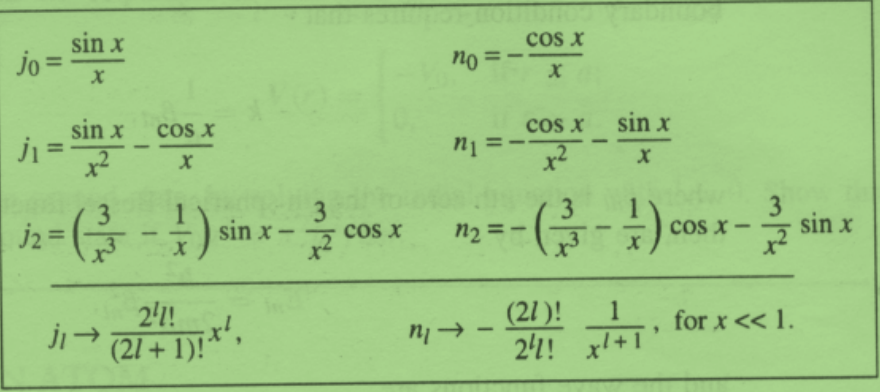
\includegraphics[width=8cm]{figure4-3.png}
        \caption{前几个Spherical Bessel 和 Spherial Neumann 函数以及x在很小时的渐进形式}
        \label{figure4.3}
    \end{figure}

    由于在原点$n_l$发散,所以我们需要$B=0$,因此
    \begin{equation}
        R(r) = Aj_l(kr)
    \end{equation}

\noindent 再考虑边界条件$R(a) = 0$,显然$k$必须满足
\begin{equation}
    j_l(ka) = 0
\end{equation}

\noindent Spherical Bessal 函数是振荡的,每个函数都有无限多个零点。不幸的是,这些零点都不是处于优美的敏感点,它们必须通过数值计算得到。
\begin{figure}[htb]
    \centering
    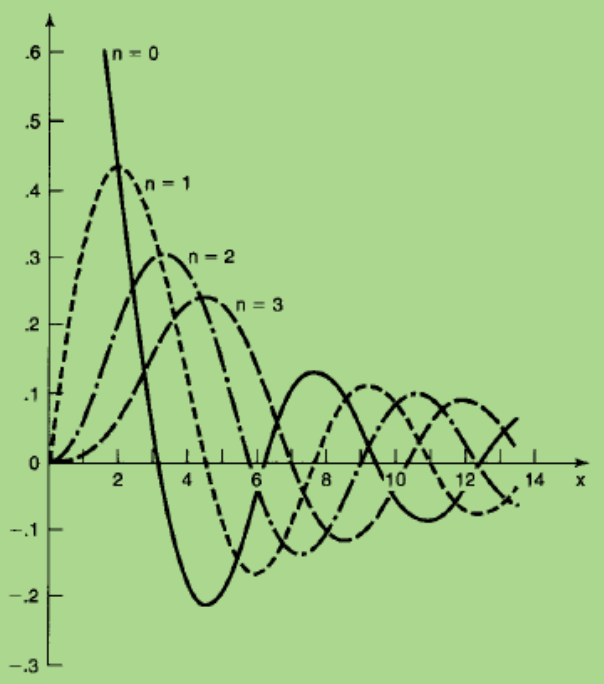
\includegraphics[width=8cm]{figure4-4.png}
    \caption{前4个Spherical Bessel 函数图}
    \label{figure4.4}
\end{figure}

    \subsection{氢原子}
    对于氢原子,径向方程可以写作
    \begin{equation}
        -\frac{\hbar^2}{2m} \frac{\mathop{}\!\mathrm{d}^2 u}{\mathop{}\!\mathrm{d} r^2} + \left[-\frac{e^2}{4 \pi \varepsilon_0} \frac{1}{r} + \frac{\hbar^2}{2m} \frac{l(l+1)}{r^2}\right] u =Eu
    \end{equation}

\noindent 定义
\begin{equation}
    \kappa = \frac{\sqrt{-2mE}}{\hbar} \label{equ4.12}
\end{equation}

\noindent 由于本问题下是束缚态,能量为负的,所以$\kappa$是实数。再引入
\begin{equation}
    \begin{aligned}
        \rho \equiv \kappa r \\
        \rho_0 \equiv \frac{me^2}{2 \pi \varepsilon_0 \hbar^2 \kappa}
    \end{aligned} \label{equ4.13}
\end{equation}

\noindent 这样有 
\begin{equation}
    \frac{\mathop{}\!\mathrm{d}^2 u}{\mathop{}\!\mathrm{d} \rho^2} = \left[1 - \frac{\rho_0}{\rho} + \frac{l(l+1)}{\rho^2}\right]u
\end{equation}

    这个时候可以先考察解的渐进形式。容易发现,当$\rho \to \infty$时,括号里的常数项其主要作用,所以得到一般解并考虑当$\rho \to \infty$时不能发散,得到
    \begin{equation}
        u(\rho) \sim Ae^{-\rho}
    \end{equation}

    另一方面当$\rho \to 0$,离心项起了主要作用,这时可以得到一般解(同样考虑到不能发散的条件)
    \begin{equation}
        u(\rho) \sim C \rho^{l+1}
    \end{equation}

    现在开始利用这两个渐进结果推出一般情况。先引入一个新的函数$v(\rho)$
    \begin{equation}
        u(\rho) = \rho^{l+1} e^{-\rho} v(\rho)
    \end{equation}

\noindent 利用这个函数时一开始显得有些繁琐
\begin{equation}
\begin{aligned} \frac{\mathop{}\!\mathrm{d}  u}{\mathop{}\!\mathrm{d} \rho} &=\rho^{\prime} e^{-\rho}\left[(l+1-\rho) v+\rho \frac{\mathop{}\!\mathrm{d} v}{\mathop{}\!\mathrm{d} \rho}\right] \\ \frac{\mathop{}\!\mathrm{d}^{2} u}{\mathop{}\!\mathrm{d} \rho^{2}} &=\rho^{\prime} e^{-\rho}\left\{\left[-2 l-2+\rho+\frac{l(l+1)}{\rho}\right] v+2(l+1-\rho) \frac{\mathop{}\!\mathrm{d} v}{\mathop{}\!\mathrm{d} \rho}+\rho \frac{\mathop{}\!\mathrm{d}^{2} v}{\mathop{}\!\mathrm{d} \rho^{2}}\right\} \end{aligned}
\end{equation}

\noindent 代入径向方程可以得到
\begin{equation}
    2(l+1-\rho) \frac{\mathop{}\!\mathrm{d} v}{\mathop{}\!\mathrm{d} \rho} + \rho \frac{\mathop{}\!\mathrm{d}^2 v}{\mathop{}\!\mathrm{d} \rho^2} + \left[\rho_0 - 2(l+1)\right]v = 0
\end{equation}

    最后我们假定$v(\rho)$可以表示为$\rho$的幂级数:
    \begin{equation}
        v(\rho) = \sum_{j=1}^{\infty} c_j \rho_j
    \end{equation}

\noindent 现在的问题是确定展开系数。逐项求导
\begin{equation}
    \begin{aligned}
        \frac{\dif v}{\dif \rho} &=\sum_{j=0}^{\infty} j c_j \rho^{j-1} = \sum_{j=0}^{\infty}(j+1)c_{j+1} \rho^j \\
        \frac{\dif^2 v}{\dif \rho^2} &= \sum_{j=0}^{\infty} j(j+1)c_{j+1}\rho^{j-1}
    \end{aligned}
\end{equation}

\noindent 代入并令同幂次项的系数相等,可以得到
\begin{equation}
    c_{j+1}=\left\{\frac{2(j+l+1)-\rho_{0}}{(j+1)(j+2 l+2)}\right\} c_{j}
    \end{equation}

    似乎工作已经完成了,存在递推公式又有办法得到从最早的$c_0$开始(它成为一个普遍乘以的常数,最后通过归一化确定),可以去玩了……但请等一下,这个递推公式无法一直作用下去,可以证明,当$j$比较大时,$u(\rho)$在递推公式(使用了近似简化运算)的帮助下会有这样的表现
    \begin{equation}
        u(\rho) c_0 \rho^{l+1} e^{\rho} 
    \end{equation}

\noindent 显然这会出现发散的情况。这看似让人很挫败,但却也因此暗藏着前进的方向。既然会出现发散,不妨就人为地将可能发散的部分干掉,于是我们试着截断这个级数,即存在某个最大的整数$j_{max}$,有 
\begin{equation}
    c_{j_{max}+1} = 0
\end{equation}

\noindent 而在在这个系数之后的所有的系数都自动为零,这显然有
\begin{equation}
    2(j_{max}+l+1) - \rho_0 =0
\end{equation}

\noindent 定义主量子数
\begin{equation}
    n \equiv j_{max} + l +1
\end{equation}

\noindent 有
\begin{equation}
    \rho_0 = 2n
\end{equation}

\noindent 根据\autoref{equ4.12}和\autoref{equ4.13}可以知道,$\rho_0$决定了能量$E$
\begin{equation}
    E = - \frac{\hbar^2 \kappa^2}{2m} = - \frac{m e^4}{8 \pi^2 \varepsilon_0^2 \hbar^2 \rho_0^2}
\end{equation}

\noindent 所以允许的能量为
\begin{equation}
    E = - \left[\frac{m}{2 \hbar^2} \left(\frac{e^2}{4 \pi \varepsilon_0}\right)^2\right] \frac{1}{n^2} = \frac{E_1}{n^2}, \qquad n=1,2,3,\cdots
\end{equation}

\noindent 这就是著名的\textbf{波尔公式},从任何程度上来说都是量子力学最重要的结果。

\noindent 其中$a = \frac{4 \pi \varepsilon_0 \hbar^2}{m e^2} = 0.529E-10\ m$ 便是所谓的\textbf{波尔半径},这样有$\kappa = \frac{1}{an}$和$\rho = \frac{r}{an}$. 

    由此得到了氢原子的空间波函数,可以用三个量子数进行标记
    \begin{equation}
        \psi_{nlm}(r,\theta,\phi) = R_{nl}(r) Y_l^m(\theta,\phi)
    \end{equation}

\noindent 其中 
\begin{equation}
    R_{nl}(r) = \frac{1}{r} \rho^{l+1} e^{-\rho} v(\rho)
\end{equation}

    虽然$v(\rho)$可以用之前的递推公式得到,但作为这么常使用的函数,显然应该有查表的可能。果不其然,它和一个特殊函数有着紧密联系,可以写作
    \begin{equation}
        v(\rho) = L_{n-l-1}^{2l+1} (2 \rho)
    \end{equation}

\noindent 其中 
\begin{equation}
    L_{q-p}^p(x) = (-1)^{p}\left(\frac{\dif}{\dif x}\right)^q L_q(x)
\end{equation}

\noindent 是缔结拉盖尔多项式(注意,不是缔结勒让德多项式,人家在球谐函数那边),其中
\begin{equation}
    L_q(x) \equiv e^x \left(\frac{\dif}{\dif x}\right)^2 (e^{-x}x^q)
\end{equation}

\noindent 是q阶拉盖尔多项式。

    由此我们终于可以一见氢原子波函数真容了,注意这里的是完整的波函数,包括了时间依赖项
    \begin{equation}
        \Psi_{n l m}=\sqrt{\left(\frac{2}{n a}\right)^{3} \frac{(n-l-1) !}{2 n[(n+l) !]^{3}}} e^{-r / n a}\left(\frac{2 r}{n a}\right)^{l}\left[L_{n-l-1}^{2 l+1}(2 r / n a)\right] Y_{l}^{m}(\theta, \phi)
        \end{equation}

\noindent 确实十分复杂,但我们得知足,因为残酷的大自然只让很少数的实际系统存在解析解,而这便是其中的一个。注意虽然波函数依赖所有的三个量子数,但是能够仅有主量子数$n$决定。这仅是库仑势所特有的,在球势阱情况下我们知道能量还依赖$l$. 所以对于氢原子系统在不考虑自旋、相对论修正等会改变其库仑势下的哈密顿量的情况下,单靠能量是无法分辨出$l,m$这两个量子数的。由球谐函数的正交性以及它们是哈密顿量算符对于不同本征值的本征函数,可以得出上面的波函数是相互正交的
\begin{equation}
    \int \Psi_{n l m}^{*} \Psi_{n^{\prime} i^{\prime} m^{\prime}} r^{2} \sin \theta \dif r \dif \theta \dif \phi=\delta_{n n^{\prime}} \delta_{l l^{\prime}} \delta_{m n^{\prime}}
    \end{equation}

    \subsubsection{氢原子光谱}
    原则上,如果把一个氢原子放到某个定态上,那么它将永远处在这个态。但是,如果给他轻微的扰动——用另一个原子撞击或者用光照射,电子就有可能跃迁到其他的定态,或者吸收能量或者释放能量。这时能量的变化便是两个态之间的能量的差值。

    可以通过波尔理论计算,也可以通过经验公式,里德伯公式进行计算。容易验证里德伯常数
    \begin{equation}
        R \equiv \frac{m}{4 \pi c \hbar^3} \left(\frac{e^2}{4 \pi \varepsilon_0}\right) = 1.097E+7/ m^{-1}
    \end{equation}

\noindent 波尔理论的巨大成就就是解释了这个公式——通过基本的自然常数计算出了R.

    \subsection{角动量}
    仿造经典下的粒子角动量(相对于原点)的定义
    \begin{equation}
        \vec{L} = \vec{r} \times \vec{p}
    \end{equation}

\noindent 当要注意对动量进行量子力学变换,由此可以得到分量形式的量子力学框架下的角动量
\begin{equation}
    \left \{ \begin{aligned}
        &\hat{L}_x =i \hbar \left(y \frac{\partial}{\partial z} -z \frac{\partial}{\partial y} \right) \\
        &\hat{L}_y =i \hbar \left(z \frac{\partial}{\partial x} -x \frac{\partial}{\partial z} \right) \\
        &\hat{L}_z =i \hbar \left(x \frac{\partial}{\partial y} -y \frac{\partial}{\partial x} \right) 
    \end{aligned} \right.
\end{equation}

    \subsubsection{本征值}
    算符$\hat{L}_x$和$\hat{L}_y$不对易,根据正则对易关系——$[\hat{x}_i,\hat{p}_j] = \delta_{ij} i \hbar$和$[\hat{p}_i,\hat{x}_j] = - \delta_{ij} i \hbar$可以得到 
    \begin{equation}
        [\hat{L}_x,\hat{L}_y] = i \hbar \hat{L}_z
    \end{equation}

\noindent 更一般地,可以得到
\begin{equation}
    \varepsilon_{ijk} \frac{[\hat{L}_i,\hat{L_j}]}{\hat{L}_k} = i \hbar  
\end{equation}

\noindent 这就是角动量的基本对易关系,其它的可由它们推出。注意这是我自创的表达方式,应该是不规范的,知道意思就好了,考试时请不要使用,或者不要把我供出来……

    由于角动量分量之间都是不相容的可观测量,由推广的不确定性原理\autoref{equ3.5}可以推得(这里只是举例,其他几个分量情况是一样的)
    \begin{equation}
        \sigma_{L_x} \sigma_{L_y} \ge \frac{\hbar}{2} |\langle L_z \rangle |
    \end{equation}

\noindent 所以寻求分量之间的共同本征函数是徒劳的。幸运的是,总角动量的平方和分量却是对易的,这里的证明需要利用一个有关对易的重要结论
\begin{equation}
    [L_i^2,L_j] = L_i[L_i,L_j]+[L_i,L_j] L_i
\end{equation}

\noindent 其中当$i=j$时右边为0. 其余的证明很简单,自己动手试试吧。由此我们可以写成更紧凑的形式
\begin{equation}
    [L^2,\vec{L}] = 0
\end{equation}

\noindent 所以可以期望找到$L^2$和$L_z$的共同本征值,这是我们使用得最多的组合——其实考虑到空间的旋转对称性,z轴的选择其实是任意的,一般选择令问题最为简化的那个方向。

    之前处理谐振子的时候利用了十分方便的“梯子算符”方法,幸运的是,角动量的求解依旧可以基本照搬那套方法,只是稍稍有些区别。先定义角动量下的“升降阶算符”,或者称为“产生-湮灭算符”
    \begin{equation}
        L_{\pm} \equiv L_x \pm i L_y
    \end{equation}

\noindent 容易证明 
\begin{equation}
    \begin{aligned}
        \left[L_z,L_{\pm}\right]&= \pm \hbar L_{\pm} \\
        [L^2,L_{\pm}]& = 0
    \end{aligned}
\end{equation}

    升降算符的定义自然不是随心所欲的,可以发现,如果$f$是$L^2$和$L_z$的共同本征函数,那么和升降算符合体之后的函数$L_{\pm}f$也是它们的共同本征函数
    \begin{equation}
        L^{2}\left(L_{\pm} f\right)=L_{\pm}\left(L^{2} f\right)=L_{\pm}(\lambda f)=\lambda\left(L_{\pm} f\right)
        \end{equation}
    
\noindent 这时对这个新的共同本征函数求$L_z$的本征值,可以发现本征值发生了变化,恰好就提升了或者降低了一个$\hbar$. 看来和谐振子那边的玩法是一样的,回忆在谐振子那边的探索,我们猜测存在一个最高的阶梯,使得
\begin{equation}
    L_{\pm} f_t = 0
\end{equation}

\noindent 这是合理的,因为$L_z$的值不能无限增大,它总会遇到一个天花板,不然它会超过角动量总量,这显然是不合理的。设$\hbar l$是$L_z$在这个最高阶梯的本征值
\begin{equation}
    \begin{aligned}
        L_z f_t &= \hbar l f_t \\
        L^2 f_t &= \lambda f_t
    \end{aligned}
\end{equation}

\noindent 因为 
\begin{equation}
\begin{aligned} L_{\pm} L_{\mp} &=\left(L_{x} \pm i L_{y}\right)\left(L_{x} \mp i L_{y}\right)\\
&=L_{x}^{2}+L_{y}^{2} \mp i\left(L_{x} L_{y}-L_{y} L_{x}\right) \\ &=L^{2}-L_{z}^{2} \mp i\left(i \hbar L_{z}\right) \end{aligned}
\end{equation}

\noindent 或者写作
\begin{equation}
    L^2 = L_{\pm} L_{\mp} + L_z^2 \mp \hbar L_z \label{equ4.7}
\end{equation}

\noindent 因此可以得到
\begin{equation}
    L^2 f_t = \hbar^2l(l+1) \Rightarrow \lambda = \hbar^2l(l+1) \label{equ4.5}
\end{equation}

    同样因为另一个方向的$L_z$不能大于总量,存在一个最小值,用同样的方法得到
    \begin{equation}
        L^2 f_b = \hbar^2\overline{l}(\overline{l}+1) \Rightarrow \lambda = \hbar^2\overline{l}(\overline{l}+1) \label{equ4.6}
    \end{equation}

\noindent 比较\autoref{equ4.5}和\autoref{equ4.6}可以得知
\begin{equation}
    l(l+1) = \overline{l}(\overline{l} -1)
\end{equation}

\noindent 数学上存在两个解,但用小学数学思维——真的应该是小学数学思维了,不是厂主的那种小学——就可以得知
\begin{equation}
    \overline{l} = - l
\end{equation}

\noindent $L_z$的本征值显然应该是$m\hbar$的形式,其中$m$从$-l$增加到$l$.

\newpage
\begin{figure}[htb]
    \centering
    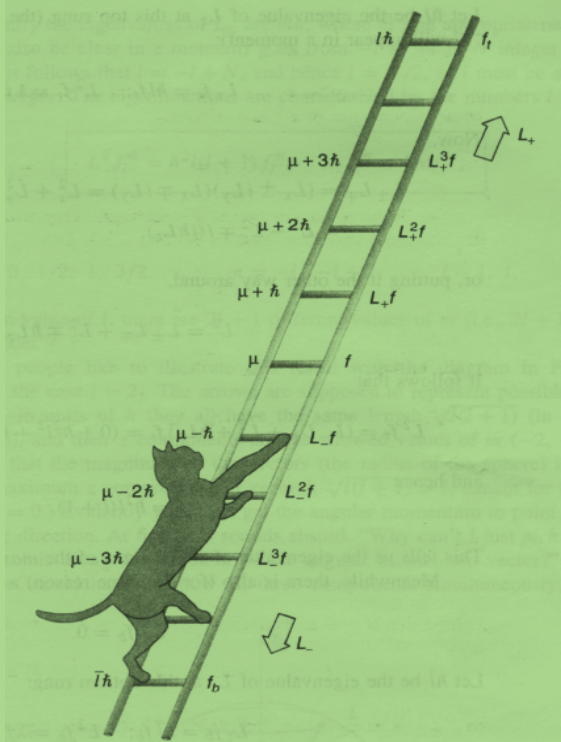
\includegraphics[width=8cm]{figure4-5.png}
    \caption{角动量的梯形式——格里菲斯书上的图,实在忍不住要放进来了。其他的就算都记不住,这张图印象贼深刻}
    \label{figure4.5}
\end{figure}

    $L_z$和$L^2$共同的本征函数需要由$l,m$这两个量子数来表征。有人喜欢用\autoref{figure4.6}来解释上面的结果。箭矢代表可能的角动量,它们的z分量是m的允许值,注意箭矢的模要比最大的$L_z$大,显然不存在完全处于$z$方向的角动量。
    \begin{figure}[H]
        \centering
        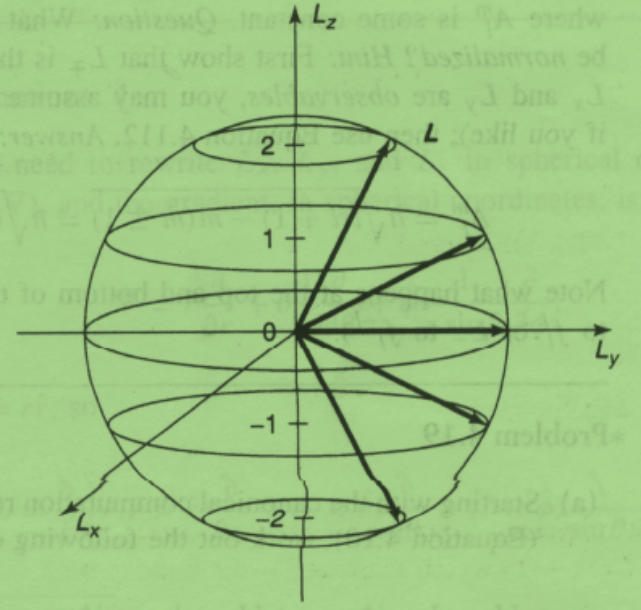
\includegraphics[width=8cm]{figure4-6.png}
        \caption{角动量态(l=2)}
        \label{figure4.6}
    \end{figure}

\noindent 可是等一下——这时有个类似厂主的方程大佬跑了出来,不过为了照顾本篇知识归纳是量子力学的,不妨就称之为“量子大佬”吧——为什么我们不能选择z方向就是沿着角动量方向呢?想了想后,你可能会有如下的解答:“在极其偶尔和幸运的情况下,这或许是可能的……”但事实上这是不可能的。由于这样做需要同时知道三个分量,但根据不确定性原理,确定了$L_z$就意味着必须放弃另外两个分量。但这还不仅仅是三个分量的问题,更关键的是——\red{一个粒子根本就不存在所谓确定的角动量矢量},就像它不存在同时确定的位置和动量一样。从这个角度上说,\autoref{figure4.6}显得容易让人误解,它应该模糊化纬度线以表示$L_x$和$L_y$是不确定的。

    下面将要开始构建本征函数,这将是一个繁杂的过程,但结果却异常亲切——$L^2$和$L_z$的共同本征函数不是别函,而恰恰就是球谐函数!由此也可以知道为什么球谐函数是相互正交的了,因为它们是厄米算符属于不同本征值的本征函数。

    \subsubsection{本征函数}
    在寻找本征函数之前,让我们先把角动量分量算符在球坐标中重新写出,对于梯度算符
    \begin{equation}
        \nabla = \hat{r} \frac{\partial}{\partial r} + \hat{\theta} \frac{1}{r} \frac{\partial}{\partial \theta} + \hat{\phi} \frac{1}{\sin \theta} \frac{\partial}{\partial \phi}
    \end{equation}
    
\noindent 另外
\begin{equation}
    \vec{r} = r \hat{r}
\end{equation}

\noindent 根据角动量算符的计算公式$\vec{L} = -i \hbar \vec{r} \times \nabla$可以得到 
\begin{equation}
    \begin{aligned}
        \vec{L}&=\frac{\hbar}{i}\left[r(\hat{r} \times \hat{r}) \frac{\partial}{\partial r}+(\hat{r} \times \hat{\theta}) \frac{\partial}{\partial \theta}+(\hat{r} \times \hat{\phi}) \frac{1}{\sin \theta} \frac{\partial}{\partial \phi}\right] \\
        &= - i \hbar \left(\hat{\theta} \frac{\partial}{\partial \theta} - \hat{\theta} \frac{1}{\sin \theta} \frac{\partial}{\partial \phi}\right)  
    \end{aligned}\label{equ4.14}
    \end{equation}

\noindent 单位矢量之间有如下转换公式(有关单位矢量之间的转换个人觉得十分重要,可以背一下,或者利用微分几何相关知识推导出来)
\begin{equation}
    \begin{aligned}
    &\hat{\theta}=(\cos \theta \cos \phi) \hat{i}+(\cos \theta \sin \phi) \hat{j}-(\sin \theta) \hat{k}\\
    &\hat{\phi}=-(\sin \phi) \hat{i}+(\cos \phi) \hat{j}
    \end{aligned}\label{equ4.8}
    \end{equation}

    将\autoref{equ4.8} 代入 \autoref{equ4.14}可以得到用直角坐标表示的角动量分量算符,但其中的依赖关系确实和球坐标下的角度相关的。这种表示充分结合了直角坐标和球坐标的优势。
    \begin{equation}
        \left \{ \begin{aligned}
            &L_x = -i \hbar \left(- \sin \phi \frac{\partial}{\partial \theta} - \cos \phi \cot \theta \frac{\partial}{\partial \phi}\right) \\
            &L_y = -i \hbar \left(+ \cos \phi \frac{\partial}{\partial \theta} - \sin \phi \cot \theta \frac{\partial}{\partial \phi}\right) \\
            &L_z = -i \hbar \frac{\partial}{\partial \phi}
        \end{aligned} \right.
    \end{equation}

    同样计算升降算符
    \begin{equation}
        L_{\pm}=L_{x} \pm i L_{y}=- i \hbar \left[(-\sin \phi \pm i \cos \phi) \frac{\partial}{\partial \theta}-(\cos \phi \pm i \sin \phi) \cot \theta \frac{\partial}{\partial \phi}\right]
        \end{equation}

\noindent 整理可得
\begin{equation}
    L_{\pm} \pm \hbar e^{\pm i \phi} \left(\frac{\partial}{\partial \theta} \pm i \cos \theta \frac{\partial}{\partial \phi}\right)
\end{equation}

\noindent 特别有 
\begin{equation}
    L_{+} L_{-}=-\hbar^{2}\left(\frac{\partial^{2}}{\partial \theta^{2}}+\cot \theta \frac{\partial}{\partial \theta}+\cot ^{2} \theta \frac{\partial^{2}}{\partial \phi^{2}}+i \frac{\partial}{\partial \phi}\right)
    \end{equation}
\noindent 注意得到这个式子时不能只是对括号里面的用$(a+b)(a-b) = a^2 -b^2$,因为括号为的$e^{\pm i \phi}$是会被$\frac{\partial}{\partial \phi}$作用的。然后利用\autoref{equ4.7}可以得到 
\begin{equation}
    L^2 = - \hbar^2 \left[\frac{1}{\sin \theta} \frac{\partial}{\partial \theta}\left(\sin \theta \frac{\partial}{\partial \theta}\right) + \frac{1}{\sin^2 \theta} \frac{\partial^2}{\partial \phi^2}\right]
\end{equation}

    现在来决定$f_l^m(\theta ,\phi)$,它是$L^2$属于本征值$h^2 l (l+1)$的本征函数 
    \begin{equation}
        L^2 f_l^m = - \hbar^2 \left[\frac{1}{\sin \theta} \frac{\partial}{\partial \theta } +\left(\sin \theta \frac{\partial}{\partial \theta}\right) + \frac{1}{\sin^2 \theta} \frac{\partial^2}{\partial \phi^2}\right] = \hbar^2 l(l+1) f_l^m \label{equ4.10}
    \end{equation}

\noindent 但这正是“角方程”。对于角向方程中的函数$f_l^m$,它也满足
\begin{equation}
    L_z f_l^m = \frac{\hbar}{i} \frac{\partial}{\partial \phi} f_l^m = \hbar m f_l^m = \hbar m f_l^m 
\end{equation}

\noindent 这个方程正好等同于方位角方程\autoref{equ4.9}. 由此可见,角动量平方算符和角动量z轴分量算符的共同本征函数(适当归一化后)便是球谐函数。加上哈密顿量,现在定态波函数是三个算符的共同本征函数(角动量算符只和角度有关,所以加上径向方程不影响本征方程的成立)。利用\autoref{equ4.10}可以把薛定谔方程写为更为紧凑的形式
\begin{equation}
    \frac{1}{2m r^2} \left[- \hbar^2 \frac{\partial}{\partial r} \left(r^2 \frac{\partial}{\partial r}\right) + L^2 \right] \psi + V \psi = E \psi   
\end{equation}

    \subsection{自旋}
    在量子力学中,自旋是一个很特别的概念,它是微观粒子的一种内在属性,不存在经典对应。因为在经典中的自旋其实就是组成物质的轨道角动量之和,但微观粒子,特别是电子是没有内在结构的,而且如果按照经典的去理解的话,表面的速度会超过光速——这显然是不可能的。自旋其实就是微观粒子的一种性质,它与空间位置无关,会像自旋一般贡献角动量,暂时如此理解就可以了。

    自旋的代数理论和轨道角动量极其相似,基本就是直接照抄
    \begin{equation}
        \varepsilon_{ijk} \frac{[S_i,S_j]}{S_k} = i \hbar 
    \end{equation}

\noindent 以及
\begin{equation}
    \left \{ \begin{aligned}
        &S^2 | s,m \rangle =\hbar^2 s (s+1) | s , m \rangle \\
        &S_z | s,m \rangle = \hbar | s, m \rangle = \hbar m |s , m \rangle
    \end{aligned} \right.
\end{equation}

\noindent 还有升降算符
\begin{equation}
    S_{\pm} |s,m \rangle = \hbar \sqrt{s(s+1) - m(m \pm 1)} | s , m \pm 1 \rangle
\end{equation}

\noindent 其中 $S_{\pm} = S_x + i S_y$

    现在本征矢不再是球谐函数——这是显然的,因为自旋和$\theta$和$\phi$并无关系。在这种情况下没有理由将$m$和$s$的半整数值排除在外。幸运的是,每一种基本粒子都有一个特定的永远不变的自旋值,不会因为扰动发生变化,相比之下,轨道角动量是会因为微扰而发生改变的。

    \subsubsection{自旋 \texorpdfstring{$\frac{1}{2}$}{Lg}}
    $s = \frac{1}{2}$是最重要的情况,因为它是构成普通物质的粒子的自旋,以及所有夸克和所有轻子的自旋。对于$s= \frac{1}{2}$,$\hat{S}^2$和$\hat{S}_z$仅有两个本征态:$\left| \frac{1}{2}, \frac{1}{2}  \right\rangle$,它被称为\textbf{上自旋态}($\uparrow$);和$\left| \frac{1}{2}, -\frac{1}{2}  \right\rangle$,被称为\textbf{下自选态}($\downarrow$)。 利用这两个基矢量,一个自旋$\frac{1}{2}$粒子的一般态可以表示成一个两元列矩阵,或称为\textbf{旋量}。
    \begin{equation}
    \chi=\left(\begin{array}{l}{a} \\ {b}\end{array}\right)=a \chi_{+}+b \chi_{-}
    \end{equation}

\noindent 其中 
\begin{equation}
    \chi_{+} = \left(\begin{array}{c}
        {1} \\ {0}
    \end{array}\right)
\end{equation}

\noindent 代表上自旋,而
\begin{equation}
    \chi_{+} = \left(\begin{array}{c}
        {0} \\ {1}
    \end{array}\right)
\end{equation}

\noindent 代表下自旋。

    另外,自旋算符可以视为$2 \times 2$的的矩阵,利用以下关系
    \begin{equation}
        \begin{aligned}
            \hat{S}^2 \chi_{+} &= \frac{3}{4} \hbar^2 \chi_{+} \\
            \hat{S}^2 \chi_{-} &= \frac{3}{4} \hbar^2 \chi_{-}
        \end{aligned}
    \end{equation}

\noindent 可以得到自旋算符的矩阵表示形式
\begin{equation}
    \hat{S}^2 = \frac{3}{4} \hbar^2 \left(\begin{array}{cc}
        {1} & {0} \\
        {0} & {1}
    \end{array}\right)
\end{equation}

    类似地可以得到
    \begin{equation}
        \hat{S}_z = \frac{\hbar}{2} \left(\begin{array}{cc}
            {1} & {0} \\
            {0} & {-1}
        \end{array}\right)
    \end{equation}

\noindent 另外根据升降算符的性质可以推得
\begin{equation}
    \hat{S}_+ = \frac{\hbar}{2} \left(\begin{array}{cc}
        {0} & {1} \\
        {0} & {0}
    \end{array}\right)
    , \qquad 
    \hat{S}_- = \frac{\hbar}{2} \left(\begin{array}{cc}
        {0} & {0} \\
        {1} & {0}
    \end{array}\right)
\end{equation}

\noindent 由于$\hat{S}_{\pm} = S_x + i S_y$,可以得到 
\begin{equation}
    \hat{S}_x = \frac{\hbar}{2} \left(\begin{array}{cc}
        {0} & {1} \\
        {1} & {0}
    \end{array}\right)
    , \qquad 
    \hat{S}_y = \frac{\hbar}{2} \left(\begin{array}{cc}
        {0} & {-i} \\
        {i} & {0}
    \end{array}\right)
\end{equation}

\noindent 由于$\hat{S}_x, \hat{S}_y$和$\hat{S}_z$都有一个因子$\frac{\hbar}{2}$,自旋算符可以更简洁地写作
\begin{equation}
    \hat{S} = \frac{\hbar}{2} \hat{\sigma}
\end{equation}

\noindent 其中 
\begin{equation}
\hat{\sigma}_{x} \equiv\left(\begin{array}{ll}{0} & {1} \\ {1} & {0}\end{array}\right), \quad \hat{\sigma}_{y} \equiv\left(\begin{array}{cc}{0} & {-i} \\ {i} & {0}\end{array}\right), \quad \quad \hat{\sigma}_{z} \equiv\left(\begin{array}{cc}{1} & {0} \\ {0} & {-1}\end{array}\right)
\end{equation}

\noindent 这就是著名的\textbf{泡利自旋矩阵}。

    $\hat{S}_z$的本征旋量就是前面的上下自旋态。如果对一个粒子的一般态测量其$S_z$,得到$\pm \frac{\hbar}{2}$的几率分别是$|a|^2$和$|b|^2$,应有 
    \begin{equation}
        |a|^2 + |b|^2 =1
        \end{equation}
    
    但是,如果测量$S_x$,可能值会是什么?按照广义的统计诠释,我们需要知道其本征值和本征旋量。可以得到其本征值为$\pm \frac{\hbar}{2}$,确实有些令人惊讶,但结果就是这样。不过本征旋量是不一样的,对于能够得到这样结果的本征旋量分别如下
    \begin{equation}
        \chi_+^{(x)} = \frac{\sqrt{2}}{2} \left(\begin{array}{c}
            {1}  \\
            {1} 
        \end{array}\right)
        , \qquad 
        \chi_-^{(x)} = \frac{\sqrt{2}}{2} \left(\begin{array}{c}
            {1} \\
            {-1} 
        \end{array}\right)
    \end{equation}

\noindent 作为厄米算符的本征矢量,它们张成空间,一般的旋量都可以表示成它们的线性叠加。根据广义统计诠释,可以知道对$S_x$进行测量得到的本征值就是该本征值对应的本征矢量的系数的平方。

    注意,对于特定的态,不能够同时测量$S_x$和$S_z$(当然包括y分量,但我现在只用这两个举例子),因为这样就违背不确定性原理了。所以特别地,对于上自旋态,我们可以很确定地说它的$S_z = \frac{\hbar}{2}$,但却没法说它其他分量的大小。我们当然可以进行测量,但不好意思,这样便对态进行干扰了,哪怕到时候得到了一个结果,态也已经坍缩到对应的本征态了,这个时候再对$\hbar$进行测量就会发现,有可能得不到之前的结果。

    在这个例子上我们可以发现,量子力学并不是说一个粒子不存在一个确定的位置、动量、角动量的z分量等等,其实在特定态它们可以是确定的,量子力学强调的是\red{观测会对物理事实(比如说态)产生显著的扰动},在这样的情况下,态已经发生了变化,对于没法同时确定的可观察量(相应的算符不对易),将没法同时得到结果,这便是不确定性的来源。

    \subsubsection{磁场中的电子}
    一个带电的自旋粒子形成一个磁偶极子,在磁场中的哈密顿量为
    \begin{equation}
        \hat{H} = - \gamma \vec{B} \cdot \vec{S}
    \end{equation}

\noindent 其中$\gamma = \frac{q}{m}$是经典值的两倍,这只有在相对论量子力学中才能得到解释。

    现在考虑磁场方向位于$z$方向,这个时候$\hat{H}$的本征矢跟$\hat{S}_z$是一样的,能量为$E_{\pm} = \mp \frac{\gamma B_0 \hbar}{2}$. 由于哈密顿量是不依赖时间的,对于含时薛定谔方程
    \begin{equation}
        i \hbar \frac{\partial \chi}{\partial t} \hat{H} \chi 
    \end{equation}

\noindent 的一般解可以表示为定态的叠加
\begin{equation}
\chi(t)=a \chi_{+} e^{-i E_{+} t / \hbar}+b \chi_{-} e^{-i E_{-} t / \hbar}=\left(\begin{array}{c}{a e^{i \gamma B_{0} t / 2}} \\ {b e^{-i \gamma B_{0} t / 2}}\end{array}\right)
\end{equation}

\noindent 常数$a,b$由初始条件决定。当然两者平方之和为1,不失一般性,令$a = \cos (\alpha/2), b = \sin (\alpha /2)$,其中$\alpha$是一个固定的角度。这样计算$\hat{S}$期待值对时间的依赖关系
\begin{equation}
\begin{aligned}\left\langle S_{x}\right\rangle&= \chi(t)^{\dagger} \hat{S}_{x} \chi(t)=\left(\cos (\alpha / 2) e^{-i \gamma B_{0} t}+2 \sin (\alpha / 2) e^{i \gamma B_{0} t / 2}\right) \\ & \times \frac{\hbar}{2}\left(\begin{array}{cc}{1} & {0} \\ {0} & {-1}\end{array}\right)\left(\begin{array}{c}{\cos (\alpha / 2) e^{i \gamma B_{0} t / 2}} \\ {\sin (\alpha / 2) e^{-i \gamma B_{0} t / 2}}\end{array}\right) \\&=\frac{\hbar}{2} \sin \alpha \cos \left(\gamma B_{0} t\right) \end{aligned}
\end{equation}

\noindent 类似可以得到 
\begin{equation}
    \begin{aligned}
        \langle \hat{S}_y \rangle &= \frac{\hbar}{2} \sin \alpha \sin (\gamma B_0 t) \\ 
        \langle \hat{S}_z \rangle &= \frac{\hbar}{2} \cos \alpha
    \end{aligned}
\end{equation}

\noindent 显然$\langle \hat{S} \rangle $ 与$z$轴有一个常数倾斜角,且绕磁场方向拉莫尔进动,频率为$\omega = \gamma B_0$,这和经典中情况一样。

    现在来看一个在量子力学中举足轻重的实验:斯特恩-格拉赫实验:一个非均匀磁场可以分离具有特定自旋指向的粒子,并且正好分为离散的许多束。 注意到除了力矩,磁偶极子还受到外一个力
    \begin{equation}
        \vec{F} = \nabla (\mu \cdot \vec{B})
    \end{equation}

\noindent 假设一束较重的中性原子(中性原子是为了避免由洛伦兹力产生的大尺度偏折,重原子是为了使我们可以构造一个局域波包,以便可以用经典的粒子轨迹处理粒子的作用——此时粒子性较为显著,容易分析)沿着y方向通过一个非均匀磁场区域
\begin{equation}
    \vec{B} (x,y,z) = - \alpha x \hat{i} + (B_0 + \alpha z) \hat{k}
\end{equation}

\noindent 其中$B_0$是一个较强的均匀场,而$\alpha$描述对均匀性的一个小的偏离。实际上我们只需要z方向上的小的偏离,但很不幸这是做不到的,$\nabla \cdot \vec{B}$使得我们必须引入x分量。但x分量和我们要讨论的问题无关。作用在原子上的力为
\begin{equation}
    \vec{F} = \gamma \alpha (-S_x \hat{i} + S_z \hat{k})
\end{equation}

    但是由于绕着$B_0$的拉莫尔进动,$S_x$快速振荡,其平均值为零,净力是沿着z轴方向,即
    \begin{equation}
        F_z = \gamma \alpha S_z
    \end{equation}
\noindent 与自旋角动量的z分量成正比,原子束向上或向下偏转。经典上,由于$S_z$没有量子化,我们预期的是一个模糊带,但实际上原子束分成了$2s+1$个分立的束,着完美地展示了角动量的量子化。
    上面的论述完全是经典的,在完全的量子计算中,没有“力”的位置,因此我们应该使用这样的描述:我们在随着原子束一同运动的参照系中来研究这个过程。在这个参考系中,哈密顿的初值为零,当粒子经过磁场的一段时间$T$内不为零,然后再归于零
    \begin{equation}
        H(t) = \left\{ \begin{array}{l}
            {0, \qquad \qquad \qquad \quad \ t<0} \\
            {(-\gamma(B_0 + \alpha z)S_z),\ 0\le t \le T}\\
            {0,\qquad \qquad \qquad \quad \  t>T}
        \end{array}\right.
    \end{equation}

\noindent 我们忽略了与问题无关的x分量。假定原子的自旋为$\frac{1}{2}$,初态为
\begin{equation}
    \chi(t) = a \chi_+ b \chi_-, \quad 0 \le t \le T
\end{equation}

\noindent 当哈密顿算符作用时,$\gamma(t)$按照通常方法演化
\begin{equation}
    \chi(t) = a \chi_+ e^{-i E_+ t / \hbar} + b \chi_- e^{-i E_- t / \hbar},\quad 0 \le t \le T
\end{equation}

\noindent 式中
\begin{equation}
    E_{\pm} = \mp \gamma (B_0+\alpha z) \frac{\hbar}{2}
\end{equation}

\noindent 因此当$t \ge T$它出现在态中
\begin{equation}
    \chi(t) = \left(ae^{i\gamma T B_0/2} \chi_+\right)e^{i(\alpha \gamma T/2)z} + \left(be^{i\gamma T B_0/2} \chi_-\right)e^{-i(\alpha \gamma T/2)z}
\end{equation}

\noindent 这两项含有沿z轴方向的动量,自旋向上的动量为
\begin{equation}
    p_z = \frac{\alpha \gamma T \hbar}{2}
\end{equation}

\noindent 方向沿着z轴正方向。自旋向下部分的动量恰好相反。因而,像上一种描述一样,原子束经过磁场分为两束,可以验证,数值结果也是一样的。

    斯特恩-格拉赫实验在量子力学的基本原理中举足轻重,它既是量子态制备的范例,又是一些量子测量的阐明模型。很多问题中我们都假设初始条件已知,但事实上该如何已知?我们可以利用斯恩特-格拉赫磁场,让未极化的粒子束通过这样的磁场,再从出射的粒子束中选择出你感兴趣的。相反地,如果想测量一个原子自旋的z分量,可以让该原子通过该装置,记录它到达接收器的位置即可。

    \subsubsection{角动量的叠加}
    假设我们有两个自旋$\frac{1}{2}$的粒子——例如,处于氢原子基态的电子和质子,简单表示为如下的形式
    \begin{equation}
        \uparrow \uparrow, \uparrow \downarrow, \downarrow \uparrow, \downarrow \downarrow
    \end{equation}

\noindent 其中第一个箭头代表电子自旋,第二个代表质子自旋。对于这个原子的总角动量,没有什么特殊的,就是两个粒子的角动量矢量叠加。上面的四个复合态的每一个都是$S_z$的一个本征态,本征值是简单的相加
\begin{equation}
\begin{aligned} S_{z} \chi_{1} \chi_{2} &=\left(S_{z}^{(1)}+S_{z}^{(2)}\right) \chi_{1} \chi_{2}=\left(S_{z}^{(1)} \chi_{1}\right) \chi_{2}+\chi_{1}\left(S_{z}^{(2)} \chi_{2}\right) \\ &=\left(\hbar m_{1} \chi_{1}\right) \chi_{2}+\chi_{1}\left(\hbar m_{2} \chi_{2}\right)=\hbar\left(m_{1}+m_{2}\right) \chi_{1} \chi_{2} \end{aligned}
\end{equation}

\noindent 因此复合系统量子数$m = m_1 + m_2$,可以有这些取值:1,0,0,-1. 

    乍一看好像有问题:m应该是以整数从$-s \to s$改变的(所以有$s=1$),但却出现了一个“额外的”$m=0$的态。搞清楚这个问题的一种方法是对态$| \uparrow \uparrow \rangle$作用降阶算符,可以得到
    \begin{equation}
    \begin{aligned} S_{-}(\uparrow \uparrow) &=\left(S_{-}^{(1)} \uparrow\right) \uparrow+\uparrow\left(S_{-}^{(2)} \uparrow\right) \\ &=(\hbar \downarrow) \uparrow+\uparrow(\hbar \downarrow)=\hbar(\downarrow \uparrow+\uparrow \downarrow) \end{aligned}
    \end{equation}

    所以其实$m=0$的情况是一个态,只不过它是叠加态,是两个本征态的线性叠加,具体位置
    \begin{equation}
        | 1 0 \rangle = \frac{1}{\sqrt{2}} \left(\uparrow \downarrow + \downarrow \uparrow\right)
    \end{equation}

\noindent 所以$s=1$的态被称为\textbf{三重态}。但需要注意,另外还有一个$| 0 0 \rangle$,这个时候的$s=0$,被称为\textbf{单重态}
\begin{equation}
    | 0 0 \rangle = \frac{1}{\sqrt{2}} \left(\uparrow \downarrow 0 \downarrow \uparrow\right)
\end{equation}

\noindent 对这个态运用升降阶算符,结果为零。

    我们的结论是,两个自旋$\frac{1}{2}$的粒子可以结合成总自旋1或0,取决于它们占据的是三重态还是单态。可以证明,三重态是$S^2$的本征值为$2 \hbar^2$的本征矢,而单态是$S^2$的本征值为0的本征矢。

    \section{旋转和角动量算符}
    \subsection{量子力学中的旋转}
    \subsubsection{无穷小旋转}
    定义无穷小旋转算符
    \begin{equation}
        \hat{R}_z(\delta \phi) \psi(r,\theta,\phi) = \psi(r,\theta,\phi) \label{equ5.1}
    \end{equation}

\noindent 对波函数使用泰勒展开
\begin{equation}
    \psi(r,\theta,\phi-\delta \phi) \approx \psi(r,\theta,\phi)- \delta \phi \frac{\partial \psi}{\partial \phi} = \left(1-\delta \phi \frac{\delta}{\delta \phi}\right) \psi(r,\theta,\phi)\label{equ5.2}
\end{equation}

\noindent 比较\autoref{equ5.1}和\autoref{equ5.2}可以得到
\begin{equation}
    \hat{R}_z(\delta \phi) = 1 - \delta \phi \frac{\delta}{\delta \phi}
\end{equation}

\noindent 又由于角动量算符
\begin{equation}
    \hat{L}_z = - i \hbar \frac{\delta}{\delta \phi}
\end{equation}

\noindent 由此得到 
\begin{equation}
    \hat{R}_z(\delta \phi) = 1 - \frac{i}{\hbar} \delta \phi \hat{L}_z\label{equ5.3}
\end{equation}

    当然这是对小角度下近似成立的。注意此时旋转轴为z轴,对于任意旋转轴
    \begin{equation}
        \hat{R}_z (\delta \phi) = 1 - \frac{i}{\hbar} \delta \phi \vec{n} \cdot \hat{L}_z
    \end{equation}

    现在来看一下旋转与对易之间的联系。仿照上面的推导,只是这次将波函数展开到二次项,以x轴为例,得到
    \begin{equation}
        \begin{aligned}
            \hat{R}_x(\delta) &= 1 - \frac{i \delta }{\hbar} \hat{L}_x - \frac{\delta^2}{2 \hbar^2}\hat{L}_x^2 \\
            \hat{R}_y(\delta) &= 1 - \frac{i \delta}{\hbar}\hat{L}_y - \frac{\delta^2}{2 \hbar^2} \hat{L}_y^2 \\
        \end{aligned}
    \end{equation}

\noindent 代入对易关系式,可以得到
\begin{equation}
    \left[\hat{R}_x,\hat{R_y}\right] = - \frac{\delta^2}{\hbar^2} \left[\hat{L}_x,\hat{L}_y\right]
\end{equation}

\noindent 可以发现有关$\delta$的一次项被消去了。同时根据经典下的旋转矩阵之间的关系(将算符写作旋转矩阵的形式,很简单便可以证明)
\begin{equation}
    \left[\hat{R}_x,\hat{R_y}\right] = \hat{R}_z(\delta^2) -1
\end{equation}

\noindent 根据\autoref{equ5.3}可以得到 
\begin{equation}
    \left[\hat{L}_x,\hat{L}_y\right] = i\hbar \hat{L}_z
\end{equation}

\noindent 用同样的方法可以推出剩下的角动量算符对易关系。

    \subsubsection{有限旋转}
    对于有限旋转,归根到底还是利用无穷小旋转加取极限操作:$\phi = N \delta \phi\ (N \to \infty)$.所以
    \begin{equation}
        \begin{aligned}
            \hat{R}_z(\phi) &= \lim_{N \to \infty} \hat{R}_z(N\delta \phi) = \lim_{N\to \infty}\left[\hat{R}_z(\delta \phi)\right]^N  \\
            &= \lim_{N \to \infty}\left(1 - i \frac{\delta \phi}{\hbar} \hat{L}_z\right)^N \\
            &=\lim_{N \to \infty}\left(1 - i \frac{ \phi}{\hbar N} \hat{L}_z\right)^N \\ 
            & = e^{- i \phi \hat{L}_z/\hbar}
        \end{aligned}
    \end{equation}

\noindent 和之前同理得到一般情况下的旋转算符表达式
\begin{equation}
    \hat{R}(\phi) = e^{-i \phi \hat{n} \cdot \hat{L}/\hbar}
\end{equation}

\noindent 目前考虑的都是无自旋系统,当考虑自旋时,角动量算符为$\hat{J} = \hat{S} + \hat{L}$
\begin{equation}
    \hat{R}_n(\phi) = e^{-i \phi \hat{n} \cdot \hat{J}/\hbar}
\end{equation}

    由此可见旋转算符取决于角动量算符。

    \subsubsection{欧拉旋转}
    欧拉旋转有三个步骤,做演示时其实是对坐标系进行旋转,但对于物体旋转道理是一样的,只是旋转方向的不同而已。注意我们使用的旋转矩阵默认正方向是逆时针,对于物体旋转时逆时针的话,根据运动的相对性,坐标系变换也就是顺时针,所以变量会差一个负号。现在假设一个xyz坐标系。
    \begin{itemize}
        \item 对xyz坐标系绕着z轴逆时针旋转$\alpha$,得到uvz坐标系
        \item 对uvz坐标系绕着v轴(即原来的y轴)旋转$\beta$,得到wvz'坐标系
        \item 最后对wvz'坐标系绕着z'轴(即原来的z轴)旋转$\gamma$,得到最终的x'y'z'轴
    \end{itemize}

\noindent 上述过程用矩阵表示如下
\begin{equation}
    \begin{aligned}
        \hat{R}(\alpha,\beta,\gamma) &= \hat{R}_{z^{\prime}}(\gamma) \hat{R}_v(\beta)\hat{R}_z(\alpha) \\
        &=\exp \left(-i\gamma \hat{J}_{z^{\prime}}/\hbar\right) \exp \left(-i\beta \hat{J}_{v}/\hbar\right) \exp \left(-i\alpha \hat{J}_{z}/\hbar\right)
    \end{aligned}
\end{equation}

    对于$\hat{J}_v$和$\hat{J}_{z^{\prime}}$,将其均写作由$\hat{J}_x,\hat{J}_y,\hat{J}_z$表示的量,首先来看$\hat{J}_v$,由矩阵变换
    \begin{equation}
        \hat{J}_v = \hat{R}_z(\alpha) \hat{J}_y \hat{R}_z(-\alpha) \label{equ5.4}
    \end{equation}

    对于这个式子的理解,有两种办法,一种我自创的(比较复杂),一种莫大佬给的(感觉比较好理解,听起来是通常的理解)。先说下我的——首先要清楚,这个等式作用的是xyz坐标系表示的右矢(如果是uwz坐标系中的,没必要改写为xyz坐标系下的算符),那实际的物理便是有一个右矢,一个和v轴相关的算符作用对它作用。为了方便理解,不失一般性,可以将$\hat{J}_v$视为$\hat{R}_v$,也就是要对这个右矢进行一个旋转操作,那该如何实现呢,毕竟还不知道如何在xyz坐标系中表示v轴。实现步骤如下
\begin{itemize}
    \item 先对xyz坐标系进行旋转操作,让其变为wvz坐标系。由于是对坐标系操作,要记得见旋转角度改为相反数
    \item 由于坐标系已经发生变化,这个时候对v旋转其实就是对y旋转,所以直接左乘上$\hat{R}_y$(或者回到题目情景是$\hat{L}_y$)
    \item 最后将坐标系归位,因为题目中并没有改变xyz坐标系,或者说,该右矢最终的表示还是xyz坐标系下的,所以再将坐标系转回来,这样便得到\autoref{equ5.4}
\end{itemize}

\noindent 莫大佬给的方法是利用坐标系变换中内积的不变性。假设作用的右矢是$|\psi^{\prime} \rangle$(注意这是在wvz坐标系下的),和自己内积即是$\langle \psi^{\prime} |\hat{L}_v| \psi^{\prime} \rangle $. 由因为对于同一个右矢,在xyz坐标系下内积应该是一样的(物理现象不因为坐标系的变换而发生改变),而$| \psi^{\prime} \rangle = \hat{R}_z(- \alpha) | \psi \rangle$(注意这里的右矢是同一个,求的是在不同坐标系下的表示,等效于坐标系旋转,要和坐标系静止而右矢旋转的情况区分开来),将这个关系代入上面的内积式就可以得到\autoref{equ5.4}.

    所以可以得到 
    \begin{equation}
        \hat{R}_v(\beta) = \hat{R}_z(\alpha) \hat{R}_y (\beta) \hat{R}_z(-\alpha) = \exp \left(-i\alpha \hat{J}_{z}/\hbar\right) \exp \left(-i\beta \hat{J}_{y}/\hbar\right) \exp \left(i\alpha \hat{J}_{z}/\hbar\right)
    \end{equation}

\noindent 同理得到
\begin{equation}
    \hat{R}_{z^{\prime}}(\gamma) = \hat{R}_v(\beta) \hat{R}_z(\alpha)\hat{R}_z(\gamma) \hat{R}_z(-\alpha)\hat{R}_v(-\beta)
\end{equation}

\noindent 经过一系列的化简后可以得到很简单的形式(注意顺序)
\begin{equation}
    \begin{aligned}
    \hat{R}(\alpha,\beta,\gamma) &= \exp \left(-i\alpha \hat{J}_{z}/\hbar\right) \exp \left(-i\beta \hat{J}_{y}/\hbar\right) \exp \left(i\gamma \hat{J}_{z}/\hbar\right) \\
        &=\hat{R}_z(\alpha) \hat{R}_y(\beta) \hat{R}_z(\gamma)
    \end{aligned}
\end{equation}

    \subsubsection{旋转算符的表示}
    由于旋转算符可以用角动量分量表示,将指数形式转变为无穷级数形式(或者用求导数的方法),再考虑对易关系,可以得到
    \begin{equation}
        \left[\hat{J},\hat{R}(\alpha,\beta,\gamma)\right] = 0
    \end{equation}

\noindent 所以 
\begin{equation}
    \begin{aligned}
        \hat{J}^2 \hat{R}(\alpha,\beta,\gamma)|j,m \rangle &= \hat{R}(\alpha,\beta,\gamma)\hat{J}^2|j,m \rangle \\
        &=j(j+1) \hat{R}(\alpha,\beta,\gamma)|j,m \rangle
    \end{aligned}
\end{equation}

\noindent $\hat{J}_z$算符没有这么好的性质,这是因为旋转算符会使态发生改变,改变后的态的$L_z$是会发生变化的。由此也可以看出,角动量的值(不是分量)在旋转下是对称的。

    考虑旋转算符对态的改变情况,由于只是在角动量分量算符作用下发生改变,可以知道态的变化应该只是量子数$m$发生改变,所以新的态为$| l ,m^{\prime} \rangle$. 同时可以这样理解,旋转算符改变了$\hat{L}_z$的取向,所以要得到新的$m$值其实就是从原来的态中抽取出属于$m^{\prime}$的那一部分,所以
    \begin{equation}
        \hat{R}(\alpha,\beta,\gamma)| j,m \rangle = \sum^{j}_{m^{\prime}=-j} |j,m^{\prime} \rangle \langle j , m^{\prime}|\hat{R} | j,m \rangle
    \end{equation}

\noindent 下面便是一堆的变量替换了,那个看起来头疼的符号就是这样出来的。先令
\begin{equation}
    D^{(j)}_{m^{\prime}m}(\alpha,\beta,\gamma) = \langle j , m ^{\prime} \rangle| \hat{R} | j ,m \rangle
\end{equation}

\noindent 由于$e^{i\alpha \hat{J}_z/\hbar} = \exp(i\alpha m) | j,m \rangle$,故
\begin{equation}
    D^{(j)}_{m^{\prime}m}(\alpha,\beta,\gamma) = e^{-i(m^{\prime}\alpha + m \gamma)} d^{(j)}_{m^{\prime}m}(\beta)
\end{equation}

\noindent 其中 
\begin{equation}
    d^{(j)}_{m^{\prime}m}(\beta) = \langle j, m^{\prime} | e^{-i\beta \hat{J}_y/\hbar} |j,m \rangle \label{equ5.5}
\end{equation}

\noindent 由此可见对m的改变主要靠的是中间那个算符。

    \autoref{equ5.5}的表达式十分复杂,请大家系好安全带
    \begin{equation}
        \begin{aligned}
            d^{(j)}_{m^{\prime}m}(\beta) &= \sum_k (-1)^{k+m^{\prime}-m} \frac{\sqrt{(j+m)!(j-m)!(j+m^{\prime})!(j-m^{\prime})!}}{(j-^{\prime}-k)!(j+m-k)!(k+m^{\prime}-m)!k!} \\
            &\times \left(\cos \frac{\theta}{2}\right)^{2j+m-m^{\prime}-2k}\left(\sin\frac{\beta}{2}\right)^{m^{\prime}-m+2k}
        \end{aligned}
    \end{equation}

\noindent $k$的取值需要保证进行阶乘的值不能为负数,而且认为$0!=1$.

    \section{不含时微扰理论}
    \subsection{一般公式表示}
    虽然通过薛定谔方程和给定势能情况下原则上可以求出所有体系的状态,但不幸的是,除了少数独特的势能以外,我们都没法精确地求解薛定谔方程(自然可以使用数值法,但有些时候我们还是想见到一些解析解,而且数值法不经过解析优化也很耗钱)。幸运的是,很多体系可以看做一些通常体系的微扰状态,而对于求解微扰体系,我们有较为成熟的理论。

    假设我们已经解出了定态薛定谔方程
    \begin{equation}
        \hat{H}^0 \psi_n^0 = E_n^0 \psi_n^0 \label{equ6.1}
    \end{equation}

\noindent 从而得到了一套完备的正交归一本征函数集$/{\psi_n^0/}$以及对应的能量本征值,现在需要考虑的是对这个哈密顿量进行一定的微小变换后,如何找到新的本征函数和本征值。请大家系好安全带,我们要开始了。

    首先,我们将哈密顿量写成两项之和
    \begin{equation}
        \hat{H} = \hat{H}^0 \lambda \hat{H}^{\prime}
    \end{equation}

\noindent 其中$\hat{H}^{\prime}$是微扰。此时,我们将$\lambda$视为很小的一个数以此来表示微扰,但在后面它更多充当一个在微分运算中进行同阶比较的工具,这个时候微扰全部由$\hat{H}^{\prime}$充当,而$\lambda=1$. 下面将$\psi_n$和$E_n$展开为$\lambda$的幂级数 
\begin{equation}
    \begin{aligned}
        \psi_n &= \psi_n^0 + \lambda \psi_n^1 +\lambda^2 \psi_n^2 + \cdots \\
        E_n &= E_n^0 + \lambda E_n^1 + \lambda^2 E_n^2 + \cdots 
    \end{aligned}\label{equ6.2}
\end{equation}

\noindent 右边第二项开始便是不同级别的修正项。将\autoref{equ6.2}代入定态薛定谔方程并将$\lambda$幂次相同的项合并。对于零级其实就是\autoref{equ6.1},这是平庸的,有意思的项是从一级开始的,为
\begin{equation}
    \hat{H}^0 \psi_n^1 + \hat{H}^{\prime} \psi_n^0 = E_n^0\psi_n^1 + E_n^1\psi_n^0 \label{equ6.3}
\end{equation}

\noindent 对于二级项有
\begin{equation}
    \hat{H}^0 \psi_n^2 + \hat{H}^{\prime} \psi_n^1 = E_n^0\psi_n^2 + E_n^1\psi_n^1 + E_n^2 \psi_n^0 \label{equ6.4}
\end{equation}

\noindent 以此类推。但目前为了过考试到这里就可以了。

    \subsubsection{一级近似理论}
    用$\langle \psi_n^0 |$与\autoref{equ6.3}进行内积运算,考虑到$\hat{H}^0$是厄米算符,存在
    \begin{equation}
        \langle \psi_n^0 | \hat{H}^0 | \psi_n^1 \rangle = \langle \hat{H}^0 \psi_n^0 | \psi_n^1 \rangle
    \end{equation}

\noindent 同时考虑到零级波函数存在的正交归一性,可以得到
\begin{equation}
    E_n^1 = \langle \psi_n^0 | \hat{H}^{\prime}| \psi_{n}^{0} \rangle
\end{equation}

    这就是一级近似理论的基本结果,在实际中也是量子力学最重要的方程,它说明\red{能量的一级修正就是微扰在非微扰态中的期待值}。对于常数微扰,一级近似修正后的能量就可以得到精确值。现在来考虑波函数的一级修正。

    先重写\autoref{equ6.3}
    \begin{equation}
        (\hat{H}^0 - E_{n}^{0}) \psi_n^1 = -(\hat{H}^{\prime} - E_n^1)\psi_{n}^{0}\label{equ6.5}
    \end{equation}

\noindent 方程右边是已知的,所以方程是关于$\psi_n^1$的非齐次微分方程。由于无微扰的波函数是完备的,所以对于$\psi_n^1$可以表示为它的线性组合
\begin{equation}
    \psi_n^1 = \sum_{m \ne n} c^{(n)}_m \psi_m^0 \label{equ6.6}
\end{equation}

\noindent 求和项没有必要包括$m=n$项,因为可以验证:如果$\psi_n^1$满足\autoref{equ6.5},那么对于任意$\alpha$,$(\psi_{n}^{1} + \alpha \psi_{n}^{0})$亦满足。将\autoref{equ6.6}代入\autoref{equ6.5},得到
\begin{equation}
    \sum_{m \ne n} (E_m^0 - E_n^0 )c^{(n)}_m \psi_m^0 = - (\hat{H}^{\prime} - E_n^1)\psi_{n}^{0}
\end{equation}

    基本的套路,取$\psi_l^0$与上式内积,当$l \ne n$,得到
    \begin{equation}
        c^{(n)}_m = \frac{\langle \psi_m^0 | \hat{H}^{\prime} | \psi_n^0}{E_n^0 - E_m^0}
    \end{equation}

\noindent 故
\begin{equation}
    \psi_n^{\prime} = \sum_{m \ne n} \frac{\langle \psi_m^0 | \hat{H}^{\prime} | \psi_n^0}{E_{n}^{0} - E_m^0} \psi_m^0
\end{equation}

\noindent 这就是非简并下的一级波函数修正。

    \subsubsection{二级能量修正}
    现在考虑\autoref{equ6.4},照例求内积和利用哈密顿算符的厄米性,得到
    \begin{equation}
        E_n^2 = \langle \psi_{n}^{0} | \hat{H} ^{\prime} | \psi_n^1 \rangle - E_n^1 \langle \psi_n^0 | \psi_n^1 \rangle  
    \end{equation}

\noindent 但注意到
\begin{equation}
    \langle \psi_n^0 | \psi_n^1 \rangle  = \sum_{m \ne n}c_m^{(n)} \langle \psi_{n}^{0} | \psi_{n}^{0} \rangle = 0 
\end{equation}

\noindent 所以可以得到
\begin{equation}
\begin{aligned} E_{n}^{2}=\left\langle\psi_{n}^{0}\left|H^{\prime}\right| \psi_{n}^{1}\right\rangle &=\sum_{n+n} \frac{\left\langle\psi_{n}\left|H^{\prime}\right| \psi_{n}^{0}\right\rangle\left\langle\psi_{n}^{0}|H| \psi_{n}^{0}\right\rangle}{E_{n}^{0}-E_{m}^{0}} \\ &=\sum_{n \neq n} \frac{\left|\left\langle\psi_{n}^{0}\left|H^{\prime}\right| \psi_{n}^{0}\right\rangle\right|^{2}}{E_{n}^{0}-E_{m}^{0}} \end{aligned}
\end{equation}

    \subsection{简并微扰理论}
    \subsubsection{二重简并}
    之前我们讨论的是非简并情况,对于简并情况需要另外的考量。先考虑最简单的二重简并情况,此时
    \begin{equation}
        \hat{H}^0 \psi_a^0 = E^0 \psi_a^0, \quad \hat{H}^0 \psi_b^0 = E^0 \psi_b^0, \quad \langle \psi_a^0 | \psi_b^0 \rangle 
    \end{equation}

\noindent 注意到$\psi_a^0$和$\psi_b^0$的线性组合也是上面的薛定谔方程的解。一般来说,微扰的作用是打破这个能量的简并,将能量分裂成两部分,如\autoref{figure6.1}所示。也可以反过来看,加入微扰后的两个态(不妨称之为“上态”和“下态”)在微扰的消除过程中能量逐步会聚,态也转变为$\psi_a^0$和$\psi_b^0$的两个线性组合。问题是,我们没法知道这两个“好的”线性组合是什么样的,这导致我们没法求出一阶能量修正量,因为我们不知道无扰动的态长什么样子。鉴于这个情况,我们把线性组合的系数代入,通过调整它们的值得到我们需要的结果。
\begin{figure}[htb]
    \centering
    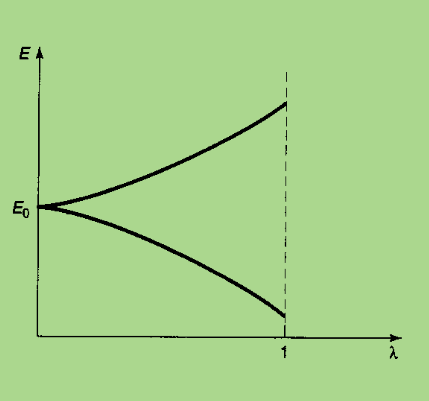
\includegraphics[width=8cm]{figure6-1.png}
    \caption{微扰使得简并能量发生分裂}
    \label{figure6.1}
\end{figure}

    和之前类似,参考\autoref{equ6.3}考虑
    \begin{equation}
        \hat{H}_0 \psi^1 + \hat{H}^{\prime} \psi^0 = E^0 \psi^1 E^1 \psi^0
    \end{equation}
\noindent 用$\psi_a^0$与上式取内积,$\hat{H}^0$为厄米算符,代入$\psi^0 = \alpha \psi$并利用正交条件得到
\begin{equation}
    \alpha \langle \psi_a^0 | \hat{H}^{\prime} | \psi_a^0 \rangle + \beta \langle \psi_a^0 | \hat{H}^{\prime} | \psi_b^0 \rangle = \alpha E^1  
\end{equation}

\noindent 写成更紧凑的形式
\begin{equation}
    \alpha W_{aa} + \beta W_{ab} = \alpha E^1 \label{equ6.7}
\end{equation}

\noindent 其中
\begin{equation}
    W_{ij} = \langle \psi_i^0 | \hat{H}^{\prime} | \psi_j^0 \rangle \quad (i,j=a,b)
\end{equation}

    类似可以得到 
    \begin{equation}
        \alpha W_{ba} + \beta W_{bb} = \beta E^1 \label{equ6.8}
    \end{equation}

\noindent 利用\autoref{equ6.7}和\autoref{equ6.8},消去$\beta W_{ab}$,在$\alpha = 0$的时候得到 
\begin{equation}
    (E^1)^2 - E^1 (W_{ab}+W_{bb}) + (W_{aa}W_{bb} - W_{ab}W_{ba}) = 0
\end{equation}

\noindent 注意有$W_{ab} = W_{ab}^*$,可以得到 
\begin{equation}
    E_{\pm}^{1} = \frac{1}{2} \left[W_{aa} + W_{bb} \pm \sqrt{(W_{aa}-W_{bb})^2 + 4|W_{ab}|^2}\right]
\end{equation}

\noindent 两个根分别对应两个受到扰动的能量。从这里也可以看出,这两个态会聚到定态的线性组合时可以为同一个线性组合。

    现在考虑$\alpha = 0$的情况,可以发现这个时候$\beta$取值任意,不如取最简单的形式$\beta = 1$,此时$W_{bb} = E^1,W_{ab}=W_{ba}=0$,所以 
    \begin{equation}
        \left \{ \begin{aligned}
            &E_+^1 = W_{bb} \langle \psi_b^0 | \hat{H}^{\prime} | \psi_b^0 \rangle \\
            &E_-^1 = W_{aa} \langle \psi_a^0 | \hat{H}^{\prime} | \psi_a^0 \rangle
        \end{aligned} \right.
    \end{equation}

\noindent 会发现这跟非简并微扰时形式一致,此时的线性关系已经是好的“线性组合”了,零级态也是“好的”态。但这只是个巧合,不过也可以因此知道,如果一开始我们就能找到“好的”零级态,我们就可以将简并微扰问题转换成非简并微扰问题来求解了。

    事实上,利用下面的定理我们总可以做到:

\noindent 如果$\hat{A}$为厄米算符,且与$\hat{H}^0$、$\hat{H}^{\prime}$都对易,又
\begin{equation}
    \hat{A} \psi_a^0 = \mu \psi_a^0, \quad \hat{A} \psi_b^0 = v \psi_b^0, \quad u \ne v
\end{equation}

\noindent 则$W_{ab}=0$,这说明$\psi_a^0$和$\psi_b^0$已经是“好的”波函数,可以直接利用非简并微扰形式求一阶能量修正。

    \subsubsection{高重简并}
    将\autoref{equ6.7}和\autoref{equ6.8}为矩阵形式
    \begin{equation}
        \begin{pmatrix}
            W_{aa} & W_{ab} \\
            W_{ba} & W_{bb}
        \end{pmatrix}
        \begin{pmatrix}
            \alpha \\
            \beta 
        \end{pmatrix}
        = E^1
        \begin{pmatrix}
            \alpha \\
            \beta 
        \end{pmatrix}
    \end{equation}

\noindent 容易发现,“好的”无微扰态的线性组合就是W矩阵的本征矢量,所以对于n重简并,通过寻找W矩阵的本征值便可以得到一阶能量修正。可以在简并的子空间里寻找一组可以使矩阵对角化的基,也可以找到那个特殊的$\hat{A}$算符,寻找满足那个定理的波函数,此时W矩阵自动对角化。

    \subsection{氢原子的精细结构}
    下面就是对推导出来的不含时微扰理论的应用。我们知道氢原子精细结构有两个来源:相对论修正和自旋-轨道耦合(这两个是完全不同的原因,但叠加得到最终的精细结构),将精细结构视为一个小的扰动,可以使用不含时微扰理论得到精细结构的结果。

    \subsubsection{相对论修正}
    动能的相对论表示式为
    \begin{equation}
        T = \frac{mc^2}{\sqrt{1-\left(\frac{v}{c}\right)^2}}
    \end{equation}

\noindent 利用动能p(注意是相对论动量)代替速度来表示$T$,则
\begin{equation}
    T = \sqrt{p^2 c^2 + m^2 c^4} - mc^2
\end{equation}

    将$\frac{p}{mc}$视为小量进行级数展开,得到最低一级相对论修正
    \begin{equation}
        \hat{H}^{\prime} = - \frac{\hat{p}^4}{8 m^3 c^2}
    \end{equation}

\noindent 根据一级近似微扰理论
\begin{equation}
    E_r^1 = \langle \hat{H}^{\prime} \rangle = - \frac{1}{8 m^3 c^2} \langle \hat{p}^2\psi | \hat{p}^2 \psi  \rangle  
\end{equation}

\noindent 由于(利用定态薛定谔方程)
\begin{equation}
    \hat{p}^2 \psi = 2m(E-V) \psi 
\end{equation}

\noindent 所以得到
\begin{equation}
    E_r^1 = - \frac{1}{2mc^2} \langle (E-V)^2 \rangle  = -\frac{1}{2mc^2}\left[E^2 - 2E\langle V \rangle +\langle V^2 \rangle \right]
\end{equation}

    这是一般情况下的。具体到氢原子中,由于
    \begin{equation}
        V(r) = - \left(\frac{1}{4 \pi \varepsilon_0}\right) e^2/r
    \end{equation}

\noindent 注意在无微扰状态下
\begin{equation}
    \begin{aligned}
        \langle \frac{1}{r} \rangle  &= \frac{1}{na^2} \\ 
        \langle \frac{1}{r^2} \rangle &= \frac{1}{\left(l+\frac{1}{2}\right) n^3 a^2}
    \end{aligned}
\end{equation}

\noindent 同时利用氢原子能级公式$E_n = -\left[\frac{m}{2\hbar^2}\left(\frac{e^2}{4 \pi \varepsilon_0}\right)^2\right] \frac{1}{n^2}$消去波尔半径a,得到 
\begin{equation}
    E_r^1 = - \frac{E_n^2}{2 m c^2} \left[\frac{4n}{l+\frac{1}{2}} - 3\right]\label{equ6.9}
\end{equation}

\noindent 可以发现,微扰的贡献相比确实很小。

    尽管氢原子有很高的简并度,但由于微扰时球对称的,因而和$L^2,L_z$对易,并且对给定的能量的$n^2$个态这些算符的本征值都不相同,波函数在这个问题上恰好是“好的”量子态,可以直接使用无简并微扰下的能量修正形式。

    \subsubsection{自旋-轨道耦合}
    取运动的电子作为参考系,可认为质子在做圆周运动(实际运动肯定不是如此,不然就违背不确定性原理了,但平均效果是这样的)形成磁场$\vec{B}$,从而有一个力矩作用于电子,使得自旋磁矩$\vec{\mu}$趋向于磁场
    \begin{equation}
        \hat{H} - \vec{\mu} \cdot \vec{B}
    \end{equation}

\noindent 对于质子磁场
\begin{equation}
    \vec{B} = \frac{\mu_0 I}{2r} = \frac{1}{4 \pi \varepsilon_0} \frac{e}{mc^2 r^3} \vec{L}
\end{equation}

\noindent 和电子磁偶极矩
\begin{equation}
    \vec{\mu_e} = - \frac{e}{m} \vec{S}
\end{equation}

\noindent 所以得到 
\begin{equation}
    \hat{H} = \left(\frac{e^2}{4 \pi \varepsilon_0}\right) \frac{1}{m^2 c^2 r^3} \vec{S} \cdot \vec{L}
\end{equation}

    由于坐标系不是惯性系,需要进行适当的动力学修正(不是重点,知道就行),引入一个$\frac{1}{2}$的因子
    \begin{equation}
        \hat{H}^{\prime} = \left(\frac{e^2}{8 \pi \varepsilon_0}\right) \frac{1}{m^2 c^2 r^3} \vec{S} \cdot \vec{L}
    \end{equation}

    由于自旋-轨道耦合的存在,哈密顿量不再与$\hat{L},\hat{S}$对易,因此自旋和轨道角动量分量不再是守恒量,取而代之的是$\hat{L}^2,\hat{S}^2$和$\hat{J} = \hat{S} + \hat{L}$. 也就是说$\hat{L}_z,\hat{S}_z$的本征态不再是“好的”本征态,而$\hat{L}^2,\hat{S}^2 \hat{J}^2$和$\hat{J}_z$才是“好的”本征态。现在
    \begin{equation}
        \hat{J}^2 = (\hat{L}+ \hat{S})^2 = \hat{L}^2 + \hat{S}^2 + 2 \hat{L} \cdot \hat{L}
    \end{equation}

\noindent 所以 
\begin{equation}
    \hat{L} \cdot \hat{S} = \frac{1}{2} (\hat{J}^2 - \hat{L}^2 - \hat{S}^2)
\end{equation}

\noindent 这个算符的本征值为$\frac{\hbar^2}{2} \left[j(j+1) - l(l+1) - s(s+1)\right]$.

    又由于 
    \begin{equation}
        \langle \frac{1}{r^3} \rangle = \frac{1}{\left(l+\frac{1}{2}\right)(l+1)n^3 a^3} 
    \end{equation}

\noindent 同样用$E_n$表示能量的一阶修正量,得到
\begin{equation}
    E^{1}=\frac{E_{n}^{2}}{m c^{2}}\left\{\frac{n\left[j(j+1)-l(l+1)-\frac{3}{4}\right]}{l\left(l+\frac{1}{2}\right)(l+1)}\right\}
\end{equation}

\noindent 和相对论修正数量级一样。两者并和,得到完整精细结构公式
\begin{equation}
    E^{1}=\frac{E_{n}^{2}}{2 m c^{2}}\left(3-\frac{4 n}{j+\frac{1}{2}}\right)
\end{equation}

\noindent 可见精细结构消除了对$l$的简并度,能量现在和$n,l$两个量子数有关了。

    \subsection{塞曼效应}
    当一个原子被置于均匀外磁场$\vec{B}_{ext}$中时,能级将发生变化,这个现象称为\textbf{塞曼效应}。与之相关的微扰量是
    \begin{equation}
        \hat{H}_{z^{\prime}} - \left(\vec{\mu}_l + \vec{\mu}_s\right) \cdot \vec{B}_{ext}
    \end{equation}

\noindent 其中与电子自旋和与轨道运动相关的磁偶极矩为
\begin{equation}
    \begin{aligned}
        \mu_s &= - \frac{e}{m} \vec{S} \\ 
        \mu_l &= - \frac{e}{2m} \vec{L}
    \end{aligned}
\end{equation}

    所以 
    \begin{equation}
        \hat{H}_{z^{\prime}} = \frac{e}{2m} (\vec{L} + 2\vec{S}) \cdot \vec{B}_{ext}
    \end{equation}

    塞塞曼效应的特性关键取决于外磁场和内磁场(自旋-轨道耦合的相对强度),较弱的视为微扰。

    \subsubsection{弱场塞曼效应}
    如果外场较弱,精细结构便是主要的,“好的”量子数为$n,l,j,m_j$(“好的”量子数即对应的算符是守恒量的量子数)。在一级微扰理论下,塞曼效应对应能量修正
    \begin{equation}
        E_z^1 = \langle \hat{H}_z^{\prime} \rangle = \langle nljm_j | \hat{H}_z^{\prime}  | nljm_j\rangle = \frac{e}{2m}\vec{B}_{ext} \cdot \langle \vec{L} + 2 \vec{S} \rangle   
    \end{equation}

\noindent 此时
\begin{equation}
    \vec{L} + 2\vec{S} = \vec{J} + \vec{S}
\end{equation}

    对于$\vec{S}$,由于总角动量为定值,$\vec{L}$和$\vec{S}$迅速绕总角动量进动,特别地,$\vec{S}$对时间的平均值恰好是它沿着$\vec{J}$的投影,即
    \begin{equation}
        \vec{S}_{ave} = \frac{(\vec{S}\cdot \vec{J})}{\vec{J}^2}\vec{J}
    \end{equation}

\noindent 又由于
\begin{equation}
    \vec{L} = \vec{J} - \vec{S}  \Rightarrow L^2 = J^2 +S^2 - 2 \vec{J}\cdot \vec{S}
\end{equation}

所以 
\begin{equation}
    \vec{J}\cdot \vec{S} = \frac{\hbar^2}{2} \left[j(j+1) - l(l+1) - s(s+1)\right]
\end{equation}

\noindent 这样得到 
\begin{equation}
    \langle \vec{L} + 2 \vec{S} \rangle = \left[1 + \frac{j(j+1)-l(l+1) + \frac{3}{4}}{2j(j+1)}\right] \langle \vec{J} \rangle 
\end{equation}

\noindent 方括号里那个常数就是著名的\textbf{朗德g系数},记做$g_j$. 特别地,如果外磁场方向就是z轴方向,可以得到
\begin{equation}
    E_z^1 = \mu_B g_j m_j B_{ext}
\end{equation}

\noindent 其中$\mu_B=\frac{e \hbar}{2m}$便是著名的\textbf{波尔磁子}。

    \subsubsection{强场塞曼效应}
    当外磁场效应远大于内磁场效应,这个时候塞曼效应是主要的了。设外磁场方向沿z轴,此时“好的”量子数为$n,l,m_l,m_s$(注意这个时候由于有外力矩的存在,总角动量不再守恒,但轨道角动量和自旋角动量分量却是守恒的)。塞曼效应哈密顿量为
    \begin{equation}
        \hat{H}_Z^{\prime} = \frac{e}{2m} B_{ext} (L_z + 2 S_z)
    \end{equation}

\noindent 无微扰时能量为
\begin{equation}
    E_{nm_lm_s} = -\frac{E_1}{n^2} + \mu_B B_{ext} (m_l + 2 m_s)
\end{equation}

\noindent 如果完全忽略精细结构的影响的话,这就是答案。但为了搞事情,加入精细结构,在一级微扰理论下,能量修正为
\begin{equation}
    E_{fs}^1 = \langle n l m_l m_s | \hat{H}_r^{\prime} + \hat{H}_{so}^{\prime} | nlm_l m_s \rangle
\end{equation}

\noindent 相对论效应还和之前一样\autoref{equ6.9},但对于自旋-轨道项却有了不同,这是因为零级态已经不同了,注意到
\begin{equation}
    \langle \vec{S} \cdot \vec{L} \rangle = \langle \hat{S}_x \rangle  \langle \hat{L}_x \rangle +\langle \hat{S}_y \rangle  \langle \hat{L}_y \rangle +\langle \hat{S}_z \rangle  \langle \hat{L}_z \rangle = \hbar^2 m_l m_s
\end{equation}

\noindent 注意现在的零级态是$S_z$和$L_z$的本征态,所以除了这两个外的期望值都为0. 经过一番复杂的运算,我们可以得到(得不到我也没办法,因为我估计我也不一定推出来,执着想推出来的可以去看格里菲斯的习题,或者去找“厂主”)
\begin{equation}
    E_{fs}^1 = \frac{E_1}{n^3} a^2 \left\{\frac{3}{4n} - \left[\frac{l(l+1)-m_lm_s}{l(l+1/2)(l+1)}\right]\right\}
\end{equation}

    和之前塞曼效应下的能量叠加起来便是总能量。

    \subsection{中间塞曼效应与超精细结构}
    简单提一下这两件事。当内外场大小相当时,需同等地将两者作为哈密顿量的扰动,这时便是中间塞曼效应。

    超精细结构是考虑了质子(或者说原子核)的自旋对磁矩的影响,使用的方法和之前是一样的。这其中存在核自旋和电子自旋的耦合,效果是打破了态的自旋简并,将三重态和单态这两种总自旋不同的情况给分离了出来。能量上抬高了三重态的能量,降低了单态的能量。
    \begin{figure}[htb]
        \centering
        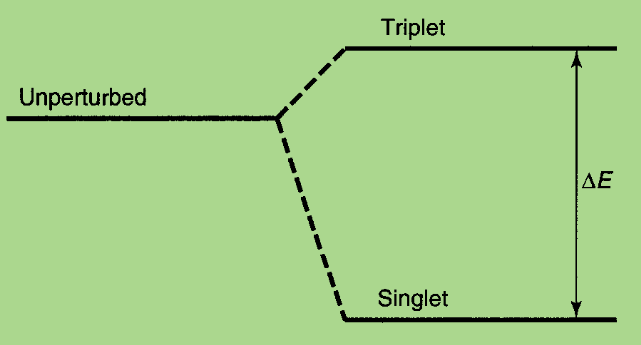
\includegraphics[width=8cm]{figure6-2.png}
        \caption{基态氢原子的超精细分裂}
        \label{figure6.2}
    \end{figure}

    \section{含时微扰论}
    到目前为止,我们考虑的量子系统的哈密顿量中的势能都是不含时的,这使得最终解出的波函数虽然还有时间项$e^{-iEt/\hbar}$,但在求概率时都会约去。所以我们一般直接求解定态薛定谔方程,这个时候几乎不用考虑时间的影响。然而,如果允许不同能级之间的跃迁,就必须引入含时势。不幸的是,只有少数这样的系统我们能够求解,但如果哈密顿量含时部分与不含时部分相比很小,我们就可以视为微扰。

    \subsection{两能级体系}
    考虑这样的两能级系统
    \begin{equation}
        \left\{\begin{aligned}
            &\hat{H}^0 \psi_a= E_a \psi_a \\ 
            &\hat{H}^0 \psi_b=E_b \psi_b
        \end{aligned}\right. \qquad 
        \langle \psi_a | \psi_b \rangle =\delta_{ab} \label{equ7.1}
    \end{equation}

\noindent 自然,更多时候系统是这样两个能级的态的线性叠加
\begin{equation}
    \Psi(0) = c_a \psi_a + c_b \psi_b
\end{equation}

\noindent 在下面的讨论中,$\Psi(t)$意味着体系在t的状态。没有微扰时,对时间的变化遵循特征指数因子变化
\begin{equation}
    \Psi(t)=c_{a} \psi_{a} e^{-i E_{a} t / \hbar}+c_{b} \psi_{b} e^{-i E_{b} t / \hbar}
\end{equation}

    \subsubsection{微扰体系}
    现在我们加上一个含时势$\hat{H}^{\prime}$,这使得$c_a,c_b$成为了时间的函数,波函数的表达式变为
    \begin{equation}
        \Psi(t)=c_{a}(t) \psi_{a} e^{-i E_{a} t / \hbar}+c_{b} \psi_{b}(t) e^{-i E_{b} t / \hbar}
    \end{equation}

\noindent 自然可以将后面的特征指数因子吸收到前面的和时间有关的函数中去,但我选择了保留。将加入了微扰的哈密顿量$\hat{H} = \hat{H}^0 + \hat{H}^{\prime}$代入含时薛定谔方程
\begin{equation}
    \hat{H} \psi = i \hbar \frac{\partial \psi}{\partial t}
\end{equation}

\noindent 得到
\begin{equation}
    \begin{aligned}
        &c_{a}\left[H_{0} \psi_{a}\right] e^{-i E_{a} t / \hbar}+c_{b}\left[H_{0} \psi_{b}\right] e^{-i E_{b} t / \hbar}+c_{a}\left[H^{\prime} \psi_{a}\right] e^{-i E_{a} t / \hbar}
        \quad+c_{b}\left[H^{\prime} \psi_{b}\right] e^{-i E_{b} t / \hbar}\\
        &=i \hbar\left[\dot{c}_{a} \psi_{a} e^{-i E_{a} t / \hbar}+\dot{c}_{b} \psi_{b} e^{-i E_{b} t / \hbar}\right. 
        \left.+c_{a} \psi_{a}\left(-\frac{i E_{a}}{\hbar}\right) e^{-i E_{a} t / \hbar}+c_{b} \psi_{b}\left(-\frac{i E_{b}}{\hbar}\right) e^{-i E_{b} t / \hbar}\right]
        \end{aligned}
\end{equation}

\noindent 根据\autoref{equ7.1}可以发现,上式左边前两项和右边后两项可以抵消,由此得到
\begin{equation}
    c_{a}\left[H^{\prime} \psi_{a}\right] e^{-i E_{a} t / \hbar}+c_{b}\left[H^{\prime} \psi_{b}\right] e^{-i E_{b} t / \hbar}=i \hbar\left[\dot{c}_{a} \psi_{a} e^{-i E_{a} t / \hbar}+\dot{c}_{b} \psi_{b} e^{-i E_{b} t / \hbar}\right]
\end{equation}

    很自然地操作,用$\langle \psi_a |$和上式进行内积操作,可以分离出$\dot{c}_a$
    \begin{equation}
        c_{a}\left\langle\psi_{a}\left|H^{\prime}\right| \psi_{a}\right\rangle e^{-i E_{a} t / \hbar}+c_{b}\left\langle\psi_{a}\left|H^{\prime}\right| \psi_{b}\right\rangle e^{-i E_{b} t / \hbar}=i \hbar \dot{c}_{a} e^{-i E_{a} t / \hbar}
    \end{equation}

\noindent 定义 
\begin{equation}
    \hat{H}_{ij}^{\prime} \equiv \langle \psi_i | \hat{H}^{\prime}| \psi_j \rangle 
\end{equation}

\noindent 容易看出,$\hat{H}_{ij}^{\prime} = (\hat{H}_{ji}^{\prime})^*$,从而可以得到
\begin{equation}
    \dot{c}_a = - \frac{i}{\hbar} \left[c_a \hat{H}_{aa} + c_b \hat{H}_{ab}^{\prime} e^{-i(E_b-E_a)t/\hbar}\right]
\end{equation}

\noindent 同理可以得到
\begin{equation}
    \dot{c}_b = - \frac{i}{\hbar} \left[c_b \hat{H}_{bb} + c_a \hat{H}_{ba}^{\prime} e^{i(E_b-E_a)t/\hbar}\right]
\end{equation}

    一般情况下,$\hat{H}_{aa}^{\prime} = \hat{H}_{bb}^{\prime} = 0$,从而可以得到
    \begin{equation}
        \left\{\begin{aligned}
            &\dot{c}_a = - \frac{i}{\hbar} \hat{H}_{ab}^{\prime} e^{-i\omega_0 t}c_b \\
            &\dot{c}_b = - \frac{i}{\hbar} \hat{H}_{ba}^{\prime} e^{i\omega_0 t}c_a 
        \end{aligned}\right.\label{equ7.2}
    \end{equation}

\noindent 其中,$\omega_0 = \frac{E_b-E_a}{\hbar}$,假定$E_b \ge E_a$.

    \subsubsection{含时微扰论}
    到现在为止推导都是严格的,现在我们引入哈密顿微扰。
    假设初始状态
    \begin{equation}
        \left\{\begin{aligned}
            &c_a(0) = 1 \\
            &c_b(0) = 0
        \end{aligned}\right.
    \end{equation}

\noindent 在没有微扰的状况,也就是零级的时候,这两个数是常数,不随时间发生变化。对于一级修正,利用\\
\autoref{equ7.2}
\begin{equation}
    \left\{\begin{aligned}
        &\dot{c}_a^{(1)} = 0 \Rightarrow \dot{c}_a^{1}(t) = 1 \\
        & \dot{c}_b^{(1)} = - \frac{i}{\hbar} \hat{H}_{ba}^{\prime} e^{i\omega_0 t} \Rightarrow c_b^{(1)}= -\frac{i}{\hbar} \int \hat{H}_{ba}^{\prime}(t^{\prime}) e^{i\omega_0 t^{\prime}} \dif t^{\prime}
    \end{aligned}\right.
\end{equation}

\noindent 继续利用\autoref{equ7.2}得到二级修正
\begin{equation}
    \left\{\begin{aligned}
        &c_a^{2}(t) = 1 - \frac{1}{\hbar^2} \int_{0}^{t} \hat{H}^{\prime}_{ab}(t^{\prime}) e^{i\omega_0 t^{\prime}}\left[\int_{0}^{t^{\prime}}e^{i \omega_0 t^{\prime \prime}}\dif t^{\prime \prime}\right] \dif t^{\prime}\\
        &c_b^{(2)}(t) = c_b^{(1)}(t)
    \end{aligned}\right.
\end{equation}

\noindent 可以发现$c_a^{(2)}$包含零阶项;积分部分是单独的二阶修正。

    一阶近似明显存在误差,因为
    \begin{equation}
        |c_a^{(1)}|^2 + |c_b^{(1)}|^2 \ne 1
    \end{equation}

\noindent 但如果对哈密顿微扰量也进行近似处理,近似到$\hat{H}^{\prime}$的一阶项,则可以满足。

    \subsubsection{正弦微扰}
    现在考虑这样的微扰
    \begin{equation}
        \hat{H}^{\prime}(\vec{r},t) = V(r) \cos (\omega t) \Rightarrow \hat{H}^{\prime} = V_{ab}\cos (\omega t)
    \end{equation}

\noindent 其中,$V_{ab} \equiv \langle \psi_a | V | \psi_b \rangle $. 这里用到了$V_{ab}= V_{ba}$,因为势能算符是个厄米算符。

    继续假设$V_{aa} = V_{bb} = 0$ 的情形,这将是遇到最多的情况,专注于一级近似,这时$c_a(t)=1$,而
    \begin{equation}
        \begin{aligned}
            c_{b}(t) & \cong-\frac{i}{\hbar} V_{a b} \int_{0}^{t} \cos \left(\omega t^{\prime}\right) e^{i \omega_{0} t} d t^{\prime}=-\frac{i V_{a b}}{2 \hbar} \int_{0}^{t}\left[e^{i\left(\omega_{0}+\omega\right) t^{\prime}}+e^{i\left(\omega_{0}-\omega\right) t^{\prime}}\right] d t^{\prime} \\
            &=-\frac{V_{a b}}{2 \hbar}\left[\frac{e^{i\left(\omega_{0}+\omega\right) t}-1}{\omega_{0}+\omega}+\frac{e^{i\left(\omega_{0}-\omega\right) t}-1}{\omega_{0}-\omega}\right]
            \end{aligned}
    \end{equation}

\noindent 看起来有些繁琐。现在我们考虑驱动频率$\omega$和跃迁频率$ \omega_0 $接近的情况,即
\begin{equation}
    \omega_0 + \omega \gg |\omega_0 - \omega|
\end{equation}

\noindent 这并不是一个不现实的限制,因为其他频率的微扰导致的跃迁概率很小。因而舍弃第一项,得到
\begin{equation}
    \begin{aligned}
        c_{b}(t) & \cong-\frac{V_{b a} e^{i\left(\alpha_{0}-\omega\right) t / 2}}{2 \hbar\left(\omega_{0}-\omega\right)}\left[e^{i\left(\omega_{0}-\omega\right) t / 2}-e^{-i\left(\omega_{0}-\omega\right) t / 2}\right] \\
        &=-i \frac{V_{b a}}{\hbar} \frac{\sin \left[\left(\omega_{0}-\omega\right) t / 2\right]}{\omega_{0}-\omega} e^{i\left(\omega_{0}-\omega\right) t / 2}
        \end{aligned}
\end{equation}

\noindent 从而得到跃迁几率
\begin{equation}
    P_{a \rightarrow b}(t)=\left|c_{b}(t)\right|^{2} \cong \frac{\left|V_{a b}\right|^{2}}{\hbar^{2}} \frac{\sin ^{2}\left[\left(\omega_{0}-\omega\right) t / 2\right]}{\left(\omega_{0}-\omega\right)^{2}}\label{equ7.3}
\end{equation}

\noindent 有意思的是,正弦微扰导致的跃迁几率随时间的变化也是正弦函数形式的,但要注意,为了保证微扰是小量的假设,计算出来的最大值
\begin{equation}
    \frac{|V_{ab}|^2}{\hbar^2 (\omega_0-\omega)^2}
\end{equation}

\noindent 必须小于一。

    \subsection{辐射的发射与吸收}
    \subsubsection{电磁波}
    辐射的发射与吸收都是和电磁场作用的,而电磁场的传递模式是电磁波。考虑到一般的电磁波的波长都远大于原子大小,所以在这个时候可以忽略场的空间变化
    \begin{equation}
        \vec{E} E_0 \cos (\omega t) \hat{k}
    \end{equation}

\noindent 所以微扰哈密顿量
\begin{equation}
    \hat{H}^{\prime} = - \mathcal{R} E_0 \cos (\omega t)
\end{equation}

\noindent 其中,$\mathcal{R} \equiv q \langle \psi_b | z | \psi_a \rangle $.

    通常$\psi$是$z$的奇、偶函数,这时$z |\psi|^2 $都为奇函数,其空间积分为零——满足$\hat{H}^{\prime}$对角元为0的通常假设。相互作用可由前面讨论的描述,注意到$V_{ab} - \mathcal{R} E_0$.

    \subsubsection{吸收、受激发射和自发发射}
    现在考虑受到单色光照射的情况,使得量子态$\psi_a \to \psi_b$,容易知道,这是正弦微扰。由\autoref{equ7.3}可知吸收概率为
    \begin{equation}
        P_{a \rightarrow b}(t)=\left(\frac{|\mathcal{R}| E_{0}}{\hbar}\right)^{2} \frac{\sin ^{2}\left[\left(\omega_{0}-\omega\right) t / 2\right]}{\left(\omega_{0}-\omega\right)^{2}}
    \end{equation}

\noindent 在这个过程中吸收能量为一个光子的能量$E = \hbar \omega_0$,我们称吸收了一个光子。还可以考虑初始态为高能态的情况($c_a^(0)=0,c_b(0)=1$),推导过程一样。或者只需要交换$a \leftrightarrow b$以及用$- \omega_0$代替$\omega_0$,最后可以得到
\begin{equation}
    P_{b \rightarrow a}(t)=\left(\frac{|\mathcal{R}| E_{0}}{\hbar}\right)^{2} \frac{\sin ^{2}\left[\left(\omega_{0}-\omega\right) t / 2\right]}{\left(\omega_{0}-\omega\right)^{2}}
\end{equation}

\noindent 这是一个令人吃惊的结果,这说明用一束光照射高能级的电子,它会跃迁到低能级,而且概率和低能级跃迁到高能级一样。这被称为\textbf{受激发射}。受激发射是激光产生的原理,但注意这必须要使绝大多数原子处于高能态。

    自发发射是这样一种现象:一个处于高能级的电子不需要任何的外部刺激就可以自发地从高能级跃迁到低能级。这是很令人奇怪的,照理说再没有扰动的情况下态是不会发生变化的。从量子电动力学的角度其实可以这样解释:自发发射本质上也是受激发射,因为基态能量不为零,高能级的电子会受到基态能量的影响,从这个角度来说,不存在真正意义上的“自发发射”,全都是“受激发射”,区别只是能量是从哪来的。

    \subsubsection{非相干微扰}
    注意到电磁场能量密度为
    \begin{equation}
        u = \frac{\varepsilon_0}{2} E^2
    \end{equation}

\noindent 所以
\begin{equation}
    P_{a \rightarrow b}(t)=\frac{2 \mu}{\varepsilon_0 \hbar^2} |R|^2 \frac{\sin ^{2}\left[\left(\omega_{0}-\omega\right) t / 2\right]}{\left(\omega_{0}-\omega\right)^{2}}
\end{equation}

    不过这只对单色光成立,在很多情况下,体系是处于一个完整频谱电磁场中的,这意味着
    \begin{equation}
        u \to \rho(\omega) \dif \omega 
    \end{equation}

\noindent 所以最终的跃迁概率密度是一个积分
\begin{equation}
    P_{a \rightarrow b}(t)=\frac{2}{\varepsilon_{0} \hbar^{2}}|\mathcal{R}|^{2} \int_{0}^{\infty} \rho(\omega)\left\{\frac{\sin ^{2}\left[\left(\omega_{0}-\omega\right) t / 2\right]}{\left(\omega_{0}-\omega\right)^{2}}\right\} d \omega
\end{equation}

\noindent 大括号中有关$\omega_0$的项为一个尖峰(出现在$\omega = \omega_0$附近),而$\rho(\omega)$通常较宽,相比起来可以认为比较均匀,所以可以用$\rho(\omega_0)$代替$\rho(\omega)$,从而提到积分号外。然后进行变量替换,即令
\begin{equation}
    x = \frac{(\omega_0 - \omega) t}{2}
\end{equation}

\noindent 对积分上下限进行扩展,在全范围内积分,这不会带来太大的影响,因为远离$\omega = \omega_0$的区域的贡献几乎为0. 这样我们可以得到
\begin{equation}
    P_{a \rightarrow b}(t) \cong \frac{\pi |R|^2}{\varepsilon_0 \hbar^2} \rho(\omega_0) t
\end{equation}

    可以发现不相干微扰成功磨平了在单色光下的跃迁概率的起伏特性,只是和时间有关,而且跃迁速率$R_{a \rightarrow b} = \frac{\dif P_{a \rightarrow b}}{\dif t}$是一个常数。


    到现在为止,微扰都只是从一个方向过来,而电场方向与传播方向垂直。然而我们需要考虑的是无特殊传播方向的电磁波和无特殊极化方向的电场。假设不同方向的入射光对场贡献相同,即$\rho(\omega)$没有方向性的差别。我们需要让
    \begin{equation}
        \overline{|\vec{\mathcal{R}}| \cdot \hat{n}^2}
    \end{equation}

\noindent 代替$|R|^2$,这里$\vec{\mathcal{R}} = q\langle \psi_a | \vec{r} | \psi_b \rangle $. 经过一番计算可以得到这种情况下的跃迁概率
\begin{equation}
    R_{a \rightarrow b}(t) = \frac{\pi}{3 \varepsilon_0 \hbar}|\vec{\mathcal{R}}|^2 \rho (\omega_0)
\end{equation}

\noindent 其中$\rho(\omega)$是$\omega_0 = \frac{E_b-E_a}{\hbar}$处单位频率间隔内场的能态密度。

    \subsection{自发发射}
    现在专门来讨论一下自发发射的问题,将其和普朗克黑体辐射公式进行对比可以发现很有趣的东西,同时可以由此得到原子物理学中的\textbf{选择定则}。
    \subsubsection{发射与吸收速率}
    假设存在低能态和高能态$\psi_a,\psi_b$,粒子数分别是$N_a,N_b$,自发发射速率为$A$,这意味着单位时间离开高能态的粒子数为$N_b A$. 由于受激发射跃迁速率与电磁场能量密度成正比(见上一节的讨论),吸收速度同样是成正比,比例系数分别为$B_{ba}$和$B_{ab}$.(我们先假设这两个比例系数不同,但后面会证明它们相同,以此验证前面得到受激发射和吸收的概率相同这一结论)

    我们得到高能态的粒子数变化速率为
    \begin{equation}
        \frac{\dif N_b}{\dif t} - N_b A - N_b B_{ba} \rho(\omega_0) + N_a B_{ba} \rho(\omega_0)
    \end{equation}

\noindent 假设系统处于热平衡状态,这个时候每一能级上的粒子数都处于动态平衡状态,即$\frac{\dif N_b}{\dif t} = 0$,所以
\begin{equation}
    \rho(\omega_0) = \frac{A}{\left(\frac{N_a}{N_b}\right)B_{ab} - B_{ba}}
\end{equation}

\noindent 当处于$T$的热平衡时,能量为$E$的粒子数目与玻尔兹曼因子成正比,所以
\begin{equation}
    \frac{N_a}{N_b} = \frac{e^{E_a/k_B t}}{e^{-E_b/k_B t}} = e^{\hbar \omega_0/k_B t}
\end{equation}

\noindent 所以
\begin{equation}
    \rho(\omega_0) = \frac{A}{ e^{\hbar \omega_0/k_B t} B_{ab} - B_{ba}} \label{equ7.4}
\end{equation}

    又因为通过普朗克黑体辐射公式可以得到热辐射能量密度为
    \begin{equation}
        \rho(\omega) = \frac{\hbar}{\pi^2 c^3} \frac{\omega^3}{e^{\hbar \omega_0/k_B t}-1}\label{equ7.5}
    \end{equation}

\noindent 通过比较\autoref{equ7.4}和\autoref{equ7.5}我们可以得到
\begin{equation}
    \left\{\begin{aligned}
        &B_{ab} = B_{ba} \\ 
        &A = \frac{\omega^3 \hbar }{\pi^2 c^3}
    \end{aligned}\right.
\end{equation}

\noindent 所以发射与吸收速率真的是一样的,而且可以将自发发射速率改写为和$\vec{\mathcal{R}}$有关的表达式
\begin{equation}
    A = \frac{\omega_0^3 |\vec{\mathcal{R}}|^2}{3 \pi \varepsilon_0 \hbar c^3}\label{equ7.6}
\end{equation}

    \subsubsection{激发态寿命}
    当对激发态注入大量粒子,由于自发发射,再时间间隔$\dif t$内,减少的粒子数为(假设无跃迁补充)
    \begin{equation}
        \dif N_b = - A N_b \dif t
    \end{equation}

\noindent 所以 
\begin{equation}
    N_b = N_b(0) e^{-At}
\end{equation}

\noindent 由此我们定义$\tau = \frac{1}{A}$为激发态的寿命。一个激发原子可以有许多衰变模,此时跃迁速度叠加
\begin{equation}
    A= A_1 + A_2 + \cdots 
\end{equation}
\noindent 故此时的寿命$\tau = \frac{1}{A_1 +A_2 + \cdots}$.

    现在来考虑一个例子。计算一个沿着x轴方向振荡的电荷q,设初态为$| n \rangle$,通过自发衰变到$| n^{\prime} \rangle$态的寿命。

    首先我们知道
    \begin{equation}
        \mathbf{\mathcal{R}} = q \langle n | x | n^{\prime} \rangle \vec{i}
    \end{equation}

\noindent 注意这里的态是谐振子态,所以有
\begin{equation}
    \langle n | x | n^{\prime} \rangle  = \sqrt{\frac{\hbar}{2 m \omega}} (\sqrt{n^{\prime}} \delta_{n,n^{\prime}-1} + \sqrt{n} \delta_{n^{\prime},n-1})
\end{equation}

\noindent 其中$\omega$是振子的固有频率。现在讨论的是自发发射,所以有$ n^{\prime} < n $,所以
\begin{equation}
    \mathbf{\mathcal{R}} = q \sqrt{\frac{n\hbar}{2m\omega}} \delta_{n^{\prime},n-1} \vec{i}
\end{equation}

\noindent 很明显,只有$n^{\prime} = n-1$是才能发生跃迁,发射频率为
\begin{equation}
    \omega_0 = \frac{E_n-E_{n^{\prime}}}{\hbar} = (n-n^{\prime})\omega =\omega 
\end{equation}

\noindent 由此得到跃迁速率
\begin{equation}
    A = \frac{nq^2 \omega^2}{6 \pi \varepsilon_0 m c^3}
\end{equation}

\noindent 和第n阶定态寿命
\begin{equation}
    \tau_n = \frac{6 \pi \varepsilon_0 m c^3}{n q^2 \omega^2}
\end{equation}

    现在我们更进一步来看一下辐射功率,并试着和经典情况下的进行比较,看能不能发现一些有意思点的东西。首先有辐射速率和每次辐射的是一个光子,能量为$\hbar \omega$可知辐射功率为
    \begin{equation}
        P_q = A \hbar \omega = \frac{q^2 \omega^2}{6 \pi \varepsilon_0 m c^3}n \hbar \omega = \frac{q^2 \omega^2}{6 \pi \varepsilon_0 m c^3}\left(E-\frac{1}{2}\hbar \omega\right)
    \end{equation}

\noindent 而对于经典情形下的同能量振子,带电量为q的粒子再加速运动时辐射功率由拉莫尔公式给出
\begin{equation}
    P_c = \frac{q^2 a^2}{6 \pi \varepsilon_0 c^3}
\end{equation}

\noindent 其中$a$为加速度。考虑到简谐振子的运动方程为$x(t) = x_0 \cos (\omega t)$,可以得到加速度为$a = - x_0 \omega^2 \cos (\omega t)$,由此并代入能量$E = \frac{1}{2} m \omega^2 x_0^2$可以得到经典辐射功率
\begin{equation}
    P = \frac{q^2 \omega^4}{6 \pi \varepsilon_0 m c^3} E
\end{equation}

    可以发现,在经典极限$\hbar \to 0$时,两者是一致的。而量子公式有一个突出的贡献,它防止了\textbf{基态辐射},即处于基态的粒子是不会发出辐射的,这是符合物理事实的。

    \subsubsection{选择定则}
    最后来考虑原子物理学一个重要的定则,并尝试从量子力学角度将其推导出来。

    由前面的讨论可以看出,计算自发速率归根到底是计算矩阵元
    \begin{equation}
        \mathcal{R}_{ba} = \langle \psi_b | \vec{r} | \psi_a \rangle 
    \end{equation}

\noindent 幸运的是,这些量常常为0. 现在来看一下什么情况下会为零,这意味着我们不需要考虑这些情况,也能够借此得到有关自发辐射的一些基本规则。由于原子中电子的态可以用三个量子数$n,l,m$表示,所以我们就用这三个量子数来标记态,得到
\begin{equation}
    \mathcal{R}_{ba} = \langle n^{\prime} l^{\prime} m^{\prime} | \vec{r} | nlm \rangle 
\end{equation}

\noindent 巧妙运动角动量算符的对易关系和厄米性会对这些量产生一些很强的限制,由此便可以得到选择定则中对于跃迁量子数的限制。

    \paragraph{有关\texorpdfstring{$m,m^{\prime}$}{Lg}的选择定则}
    考虑以下角动量对易关系
    \begin{equation}
        \left[L_{z}, x\right]=i \hbar y, \quad\left[L_{z}, y\right]=-i \hbar x, \quad\left[L_{z}, z\right]=0
    \end{equation}

\noindent 先考虑第三个,有
\begin{equation}
    \begin{aligned}
        0&=\left\langle n^{\prime} l^{\prime} m^{\prime}\right|\left[L_{z}, z\right] |n l m\rangle=\left\langle n^{\prime} l^{\prime} m^{\prime}\left|L_{z} z-z L_{z}\right| n l m\right\rangle \\
        &=\left\langle n^{\prime} l^{\prime} m^{\prime}\left|\left[\left(m^{\prime} \hbar\right) z-z(m \hbar)\right]\right| n l m\right\rangle\\
        &=\left(m^{\prime}-m\right) \hbar\left\langle n^{\prime} l^{\prime} m^{\prime}|z| n l m\right\rangle
        \end{aligned}
\end{equation}

\noindent 这表明,要不$m \ne m^{\prime}$,要不矩阵元$\langle n ^{\prime} l ^{\prime} m^{\prime} | z|nlm \rangle =0$.

    同样的,从第一和第二个对易关系可以得到(中间过程省略)
    \begin{equation}
        \begin{aligned}
            \left(m^{\prime}-m\right)\left\langle n^{\prime} l^{\prime} m^{\prime}|x| n l m\right\rangle&= i\left\langle n^{\prime} l^{\prime} m^{\prime}|y| n l m\right\rangle \\
            \left(m^{\prime}-m\right)\left\langle n^{\prime} l^{\prime} m^{\prime}|y| n l m\right\rangle&= -i\left\langle n^{\prime} l^{\prime} m^{\prime}|x| n l m\right\rangle
        \end{aligned}
    \end{equation}

\noindent 所以得到 
\begin{equation}
    (m^{\prime} - m)^2 \left\langle n^{\prime} l^{\prime} m^{\prime}|x| n l m\right\rangle = \left\langle n^{\prime} l^{\prime} m^{\prime}|x| n l m\right\rangle
\end{equation}

\noindent 同理也可以得到有关y的类似的式子。综合上面的讨论,得到有关$m$的跃迁选择定则:\red{除非$\Delta m = 0 , \pm 1$,否则没有跃迁发生}。

    \paragraph{有关\texorpdfstring{$l,l^{\prime}$}{Lg}的选择定则}
    考虑对易关系 
    \begin{equation}
        \left[L^2,\left[L^2,\vec{r}\right]\right] = 2 \hbar^2 (\vec{r}L^2 + L^2 \vec{r})
    \end{equation}

\noindent 则
\begin{equation}
    \left\langle n^{\prime} l^{\prime} m^{\prime}|\left[L^2,\left[L^2,\vec{r}\right]\right]| n l m\right\rangle= 2 \hbar^2 \left\langle n^{\prime} l^{\prime} m^{\prime}|\vec{r}L^2 + L^2 \vec{r}| n l m\right\rangle = 2 \hbar^4 \left[l(l+1) + l^{\prime}(l^{\prime}+1) \right]\left\langle n^{\prime} l^{\prime} m^{\prime}|\vec{r}| n l m\right\rangle
\end{equation}

\noindent 又因为
\begin{equation}
    \begin{aligned}
        \left\langle n^{\prime} l^{\prime} m^{\prime}|\left[L^2,\left[L^2,\vec{r}\right]\right]| n l m\right\rangle &= \left\langle n^{\prime} l^{\prime} m^{\prime}|\left[L^2\left[L^2,\vec{r}\right] - \left[L^2,r\right]L^2\right]| n l m\right\rangle \\
        &= \hbar^2 \left[l^{\prime}(l^{\prime}+1) - l(l+1)\right]\left\langle n^{\prime} l^{\prime} m^{\prime}|\left[L^2,\vec{r}\right]| n l m\right\rangle \\
        &=\hbar^4 \left[l^{\prime}(l^{\prime}+1) - l(l+1)\right]^2 \left\langle n^{\prime} l^{\prime} m^{\prime}|\vec{r}| n l m\right\rangle
    \end{aligned}
\end{equation}

\noindent 由此可知,要不$2\left[l(l+1)+l^{\prime}\left(l^{\prime}+1\right)\right]=\left[l^{\prime}\left(l^{\prime}+1\right)-l(l+1)\right]^{2}$,要不$\left\langle n^{\prime} l^{\prime} m^{\prime}|\vec{r}| n l m\right\rangle = 0$.

    对于第一个等式,可以得到三个解$\Delta l=0(l=l^{\prime}=0),\pm1$,但第一个解是不成立的,原因是当$l = l^{\prime} = 0$时,可以证明矩阵元
    \begin{equation}
        \left\langle n^{\prime} l^{\prime} m^{\prime}|\vec{r}| n l m\right\rangle = 0
    \end{equation}

\noindent 所以得到有关$l$的选择定则:\red{除非$\Delta l = \pm 1$,否则不发生跃迁}。
\end{document}
